\documentclass[fleqn,10pt,lineno]{wlpeerj}
\usepackage{amssymb}
\usepackage{amsmath}
\usepackage{url}
\usepackage{xspace}
\usepackage{caption}
\usepackage{subcaption}
\usepackage{algorithm}
\usepackage{algpseudocode}
\usepackage{xcolor}
\usepackage{tcolorbox} 
\tcbuselibrary{breakable}
\newtcolorbox[auto counter
%,number within=section
]{mybox}[2][]{
title=Box~\thetcbcounter: #2,#1,
colback=white,
colframe=gray,
fonttitle=\bfseries,
parbox=false
}
\usepackage{enumitem}


\title{Bi-objective trail-planning for a robot team orienteering in a hazardous environment}
\author[1]{Cory M. Simon$^*$}
\author[2]{Jeffrey Richley}
\author[2]{Lucas Overbey$^\ddagger$}
\author[2]{Darleen Perez-Lavin$^\dagger$}
\affil[1]{School of Chemical, Biological, and Environmental Engineering. Oregon State University. Corvallis, OR. USA.}
\affil[2]{Naval Information Warfare Center Atlantic. Charleston, SC. USA.}
 \corrauthor[1]{Cory M. Simon}{cory.simon@oregonstate.edu}


%\flushbottom
% \maketitle
%\thispagestyle{empty}


%\affil[*]{}
% \date{}							% Activate to display a given date or no date

\begin{abstract}
Consider a team of mobile [aerial, ground, or aquatic] robots for orienteering in a hazardous environment. Modeling the environment as a directed graph, each arc is labeled with a probability that a robot will survive upon traversing it, and each node is labeled with the reward given to the robot team if visited by a robot. The arc-traversal hazards could emanate from e.g.\ rough terrain or seas, strong winds, radiation, or adversaries capable of attacking or capturing robots. Each reward represents the utility gained by the team when a robot e.g.\ delivers a good, takes an image or measurement, or actuates some process to/of/at a node. We want to obtain the Pareto-optimal set of robot-team trail plans on this graph that maximize two [conflicting] team objectives: the expected (1) team reward and (2) number of robots that survive the mission. This way, a human decision-maker can inspect the reward-survival tradeoffs along the Pareto-front, then make an informed selection of a Pareto-optimal robot-team trail plan that balances, according to his or her values, reward and robot survival.  To search for the Pareto-optimal set of robot-team trail plans, we implement bi-objective ant colony optimization, guided by both pheromone and problem-specific heuristics. We solve and analyze three problem instances: a synthetic one on a two-community graph; an information-gathering mission in an art museum; and an item-tagging and -verification mission at an abandoned nuclear power plant. We find that ant colony optimization consistently outperforms or performs indistinguishably from a simulated annealing baseline. Ablating the pheromone trails or heuristics reveals that both are important for guiding ants towards Pareto-optimal robot-team trail plans. By inspecting a sample of Pareto-optimal robot-team trail plans along the Pareto-front, we find robots take the safest trails to visit the nodes assigned to them and visit higher-reward nodes earlier in their trail; multiple robots may plan to redundantly visit the same subgraphs to make the team reward robust to robot failures; and rewards from visiting nodes must be balanced against robot survival.
\end{abstract}

\begin{document}

\flushbottom
\maketitle
\thispagestyle{empty}



\clearpage


\section{Introduction}
\subsection{Applications of a team of mobile robots}
Mobile [aerial \cite{leutenegger2016flying}, ground \cite{chung2016wheeled}, or aquatic \cite{choi2016underwater}] robots equipped with sensors, actuators, and/or cargo have applications in agriculture 
% (e.g.\ planting and harvesting crops, spraying pesticide, monitoring crop health, destroying weeds) 
\cite{santos2020path,bawden2017robot,mcallister2018multi}, 
commerce % (e.g.\ order fulfillment in warehouses)
 \cite{wurman2008coordinating}, 
the delivery of goods \cite{coelho2014thirty}, 
search-and-rescue \cite{queralta2020collaborative,rouvcek2020darpa}, 
CBRN (chemical, biological, radiological, or nuclear) hazard mapping and localization %(e.g.\ safely localizing the source(s) and mapping the distribution of the hazard)
 \cite{murphy2012projected,hutchinson2019unmanned}, 
 environmental monitoring \cite{dunbabin2012robots,hernandez2012mobile,yuan2020maritime,apprill2023toward}, 
 inspection of infrastructure \cite{lattanzi2017review},
 process monitoring in industrial chemical plants \cite{soldan2014towards,francis2022gas}, 
 forest fire monitoring and fighting \cite{merino2012unmanned}, 
 wildlife conservation \cite{kamminga2018poaching},
 patrolling \cite{basilico2022recent},
 target tracking \cite{robin2016multi,hausman2016occlusion}, and 
 military surveillance and reconnaissance. 
 
Algorithms for both low-level, tactical planning and high-level, strategic planning of the paths/routes of mobile robots in [static or dynamic; known or uncertain] environments \cite{lavalle2006planning,liu2023path,ugwoke2025simulation,siegwart2011introduction,patil2012estimating,van2016motion} are vital for autonomy and pivotal for efficiency, safety, and good performance on the objectives.

The classic, low-level path-planning problem for a robot \cite{lavalle2006planning,agrawal2022classical} involves finding the least-cost (e.g., shortest), collision-free path from a starting location to a destination in a static, known environment containing obstacles.
% modeled as a grid, where obstacles render some grid cells inaccessible.
By discretizing the environment with a cell decomposition method \cite{latombe2012robot}, we can model the environment as a graph, where nodes represent locations and edges represent traversable connections between locations. Then, a variety of graph search (e.g., Dijkstra's algorithm \cite{candra2020dijkstra}), random sampling (e.g., rapidly exploring random trees \cite{lavalle1998rapidly}), heuristic (e.g., A-star \cite{candra2020dijkstra}), meta-heuristic (e.g., ant colony optimization \cite{brand2010ant}), and reinforcement learning \cite{singh2023review} algorithms can be adopted for finding a low-cost, collision-free path in this graph. 
The selection of a path-planning algorithm involves tradeoffs in solution quality, computational cost, memory usage, parallelizability, and scalability \cite{ugwoke2025simulation}.
In multi-robot path-planning \cite{wagner2011m}, each robot has unique start and end locations; robot-robot collisions must be avoided as well as robot-obstacle collisions; and the configuration space is much larger.
In multi-objective robot path-planning \cite{tarbouriech2020bi,jimenez2024exploring,ntakolia2022comparative,dao2016multi,thammachantuek2022path}, a tradeoff between the length of the path and e.g.\ the energy expenditure of the robot to take the path (encouraging smoothness) must be met.

For many applications, we wish for a team of multiple mobile robots to coordinate their routes in an environment to cooperatively achieve a shared, high-level objective \cite{parker1995design,parker2007distributed}. 
Compared to a single robot, a coordinating robot team can increase spatial coverage, enhance performance on the objective, achieve the objective more quickly, and make achievement of the objective robust to the failure of some robots \cite{schranz2020swarm,brambilla2013swarm}.
Multi-robot, coordinative route-planning involves high-level, strategic decision-making; fine-grained details like obstacle avoidance and the exact paths in Euclidean space are delegated to lower-level decision-making systems. 
Typically, such a multi-robot, coordinative routing problem is framed as a combinatorial optimization problem.

%, framed as a combinatorial optimization problem,
% Multi-robot, coordinative routing problems are framed as combinatorial optimization problems.
A prominent example of multi-robot, coordinative route-planning is the team orienteering \cite{golden1987orienteering} problem (TOP) \cite{chao1996team,gunawan2016orienteering,vansteenwegen2011orienteering}.
In the TOP, a team of robots are mobile in an environment modeled as a graph, and each node gives a reward to the team if visited by a robot.
The TOP is to plan the routes of the robots, from a source to destination node, to gather the most rewards as a team under a travel budget for each robot. 
Loosely, the TOP problem combines aspects of the classic knapsack problem (selecting the nodes from which to collect rewards, under the travel budget) and the traveling salesman problem (finding the shortest path that visits these nodes) \cite{vansteenwegen2011orienteering}.
The TOP can be formulated as an integer program.
Approaches to obtain a solution to the TOP include exact (e.g., a branch-and-price scheme \cite{boussier2007exact}), heuristic \cite{chao1996team}, and meta-heuristic (e.g., ant colony optimization \cite{ke2008ants}) algorithms \cite{vansteenwegen2011orienteering}. Again, algorithm selection involves tradeoffs in solution quality and computational efficiency. 

\subsection{Teams of mobile robots orienteering in hazardous environments} 
In some applications, robots move in a hazardous environment \cite{trevelyan2016robotics,trevelyan2016robotics} and incur spatially-inhomogeneous risks of failure, destruction, disablement, and/or capture. 
These uncertain hazards could originate from dangerous terrain, rough seas, strong winds, extreme temperatures, radiation, corrosive chemicals, or mines---or, an adversary with the capability to attack and destroy, disable, or capture robots \cite{agmon2017robotic}. 

Robots traversing a hazardous environment should plan and coordinate their routes in consideration of risks of failure.
First, each robot should take the safest route to visit its destination(s). 
Second, the robots should collaborate when planning their routes to make achievement of the team objective resilient to robot failures \cite{zhou2021multi}. 
A \emph{resilient} team of robots \cite{prorok2021beyond}
(i) anticipates failures and makes risk-aware route plans that endow the team with \emph{robustness}---the ability to withstand failures with minimal concession of the objective---e.g., by redundantly assigning multiple robots to a task requiring only one robot,
and/or
(ii) adapts their route plans during the mission in response to realized robot failures to recoup the otherwise anticipated loss in the objective. 
Third, the route plans must balance the rewards gained from visiting different locations against the risks incurred by the robots to reach those locations.
Notably, classical robot path-planning algorithms have been extended to handle environments containing uncertain hazards by minimizing two conflicting objectives: the length of the path and the robot's exposure to hazards (radiation, landmines, etc.) along the path \cite{zhang2023multi,zhang2013robot,cui2023improved}.

A few route-planning problems for robots orienteering in hazardous environments, abstracted as graphs, have been framed and solved \cite{zhou2021multi}. 
In the Team Surviving Orienteers problem (TSOP) \cite{jorgensen2018team,jorgensen2017matroid,jorgensen2024matroid}, each node of the graph offers a reward to the team when visited by a robot, and a robot incurs some probability of destruction with each edge-traversal.
The objective in the TSOP is to plan the paths of the robots, from a source to destination node, to maximize the expected team reward. As constraints, each robot must survive the mission with a probability above a tolerable threshold. 
In the \emph{offline} TSOP, the paths of the robots are set at the beginning of the mission, then followed without adaptation; in the \emph{online} setting, the paths are updated during the mission in response to realized robot failures.
%In the extended Matroid TSO problem \cite{jorgensen2017matroid,jorgensen2024matroid}, we seek to maximize the weighted
%expected number of nodes visited by one or more robots.
Relatedly, the Foraging Route with the Maximum Expected Utility problem \cite{di2022foraging} is to plan the foraging route of a robot collecting rewards in a hazardous environment, but the rewards are lost if the robot is destroyed before returning to the source node to deposit the goods it collected.
In the Robust Multiple-path Orienteering Problem (RMOP) \cite{shi2023robust}, similarly, each node gives a reward to the team only if a robot visits it \emph{and} survives the mission to deposit the reward. The paths of the $K$ robots, subject to travel budgets, are planned to maximize the team reward under the worst-case attacks of $\alpha<K$ of the robots by an adversary. 
The offline version of the RMOP constitutes a two-stage, sequential game with perfect information: (1) the robot team chooses a set of paths then (2) the adversary, knowing these paths, chooses the subset of robots to attack and destroy. 
The optimal path plans for the robots must trade (i) redundancy in the nodes visited, to give robustness against attacks, and (ii) coverage of many nodes, to collect many rewards.
In the hazardous orienteering problem (HOP) \cite{santini2023hazardous,montemanni2025exact}, robots incur a risk of destruction while carrying valuable parcels picked up at some nodes, and the reward is received iff the robot returns safely to the depot node.
Notably, Subramanian (1997) was perhaps the first to model stochastic hazards encountered by a robot taking a path on a graph \cite{sherali1997low}.
Other work involving robots traversing hazardous environments includes 
maximizing coverage of an area containing threats to robots \cite{korngut2023multi,yehoshua2016robotic}, 
handling adversarial attacks on the sensors of the robots \cite{liu2021distributed,zhou2022distributed,mayya2022adaptive,zhou2018resilient}, 
gathering information in an environment with unknown hazards \cite{schwager2017multi},
finding the optimal formation for a robot team \cite{shapira2015path},
and 
multi-robot patrolling under adversarial attacks \cite{huang2019survey}.
Though not a robot routing problem, the time-bomb knapsack problem \cite{monaci2022exact} is relevant to robots carrying hazardous cargo or cargo that invites attacks: maximize the expected profit of items placed in a knapsack under a capacity when each item has a probability of exploding and causing the profit to be lost.

\subsection{Our contribution}
Herein, our contribution is:
(1) framing and intuiting a bi-objective variant of the offline TSOP \cite{jorgensen2018team,jorgensen2017matroid,jorgensen2024matroid}, the bi-objective team orienteering in hazardous environments (BOTOHE) problem, then 
(2) specifying, implementing, and benchmarking a bi-objective ant colony optimization algorithm \cite{iredi2001bi}, guided by BOTOHE-specific heuristics, to search for the Pareto-optimal set of robot-team trail plans, then
(3) solving and analyzing BOTOHE problem instances on synthetic and real-world graphs for insights.

In the BOTOHE problem, 
%Then, we use a bi-objective ant colony optimization algorithm, guided by heuristics, to search for the Pareto-optimal robot-team trail plans.
%For illustration, we solve a BOTOHE instance for an information-gathering mission in an art museum. % nuclear power plant in a Defense Advanced Research Projects Agency (DARPA) robots challenge.
% \paragraph{The bi-objective team orienteering in hazardous environments problem (BOTOHE).} 
a team of robots are mobile in a hazardous environment, modeled as a directed graph where each arc presents a known probability of destruction to a robot that traverses it.
Each node of the graph gives a reward to the team if visited by a robot.
The robots begin at a source node.
The BOTOHE problem is to plan the closed trails of the robots to maximize two team-level objectives: the expected
(1) rewards accumulated by the team and
(2) number of robots that survive the mission. 
See Fig.~\ref{fig:overview}.
(We focus on the offline setting, corresponding with a lack of communication with/between robots after the mission executes.)


Three interesting features of the BOTOHE are: 
(1) for the survival objective, robots a) risk-aversely avoid visiting dangerous subgraphs despite rewards offered by nodes therein and b) take the safest closed trails to visit the nodes assigned to them;
(2) for the reward objective, the robots a) daringly visit dangerous subgraphs to attempt collection of the rewards offered by nodes therein, b) visit the lower-risk and higher-reward subgraphs earlier in their trails, and c) build node-visit redundancy into their trail plans (i.e., multiple robots plan to visit the same node despite zero marginal reward for a second, third, and so-on visit) to make the team-reward robust to the loss of robots during the mission; and
(3) comparing (1a) and (2a), the two objectives are inherently conflicting, as the robots must risk their survival while taking their trails to visit nodes and collect rewards.%\footnote{Two extremes: (1) to maximize survival, the robots never leave the base node no matter the rewards to be gained and (2) to maximize reward, each robot traverses the entire graph no matter the risks involved.}.

To handle the conflict between the reward and survival objectives in the BOTOHE, we search for the Pareto-optimal set \cite{pardalos2017non,branke2008multiobjective} of robot-team trail plans. By definition, a Pareto-optimal robot-team trail plan cannot be altered to give a higher expected reward without lowering the expected number of robots that survive---and vice versa. The Pareto front is the set of expected (rewards, survivals) objective vectors corresponding with the Pareto-optimal set of robot-team trail plans.
Fig.~\ref{fig:pareto_optimal} illustrates.
As opposed to aggregating the two objectives into a single, scalar objective, a Pareto front (i) reveals the tradeoffs between expected rewards and robot survivals and (ii) allows us to delay placement of quantitative preferences on each of the two objectives.
Later, a human decision-maker presented with the Pareto-front can examine the tradeoffs then make an informed selection of a Pareto-optimal robot-team trail plan that suites their preferences/values at the moment.
E.g., for a team of aerial robots on a covert information-gathering mission in an adversarial environment, a human must choose how to balance (a) the utility gained from obtaining images of the locations of interest with (b) the possible loss of [expensive] robots due to attacks.

To search for the Pareto-optimal set of robot-team trail plans in the BOTOHE, we specify, implement, and benchmark a bi-objective ant colony optimization (ACO) algorithm \cite{iredi2001bi}, guided by heuristics.
We adopt the ACO meta-heuristic \cite{dorigo2006ant,bonabeau1999swarm,blum2005ant} for the BOTOHE for several reasons.
Generally, ACO, a swarm intelligence method, excels at searching for [near-]optimal trails on graphs.
In ACO, a simulated colony of decentralized ants constructs trails stochastically and iteratively while 
(1) collectively learning from feedback (i.e., computed objective values associated with trails they construct) by laying pheromone on their constructed trails in proportion to their quality (i.e., objective value) and
(2) during trail construction, balancing 
(a) exploitation of the colony's memory of good trails via biasing towards taking arcs with high pheromone and 
(b) exploration of new trails via stochasticity and pheromone evaporation.
(As the search proceeds, the colony gradually switches from exploration to exploitation.)
Advantageously, ACO allows us to incorporate TOHE-specific heuristics to bias ants' trail construction in the beginning of the search and accelerate convergence.
ACO handles our bi-objective problem by (1) assigning ants to specialize to different regions of the Pareto front and (2) maintaining two species of pheromone---one for each objective---on the arcs \cite{iredi2001bi}.
Finally, ACO is computationally efficient (compared to integer program solvers \cite{pascariu2021train}), straightforward to implement, embarrassingly parallelizable (allocate one ant per thread), and likely extendable to efficiently handle dynamic or online BOTOHE problem variants via exploiting the knowledge stored in the pheromone trail for a warm start to the modified problem \cite{montemanni2005ant,angus2005dynamic,leguizamon2013ant,mavrovouniotis2020ant}.

For illustration, we solve and analyze a series of three BOTOHE problem instances:
(1) a synthetic, two-community graph with random node-rewards and arc-survival-probabilities;
(2) an information-gathering mission in the San Diego art museum;
and
(3) a mission to tag or verify items in the [unfinished] Satsop Nuclear Power Plant used for the Defense Advanced Research Projects Agency (DARPA) Subterranean Robotics Challenge \cite{ackerman2022robots,orekhov2022darpa}.
For each problem, we visualize and discuss
(A) the problem setup (graph; rewards, survival probabilities, robot team start); 
(B) the search progress of ACO in terms of the area under the Pareto-front of robot-team trail plans as a function of iterations;
(C) the Pareto-front at the end of an ACO run along with a sample of three Pareto-optimal robot-team trail plans; and
(D) the pheromone trails at the end of an ACO run.
Further, we quantify the contribution of (a) the greedy heuristics and (b) the pheromone to the search efficiency of ACO through two ablation studies. Diminished search efficiency upon ablation revealed that both the heuristics and pheromone are important for guiding ants towards Pareto-optimal robot-team trail plans.
We also benchmark bi-objective ACO against (a) random search and (b) bi-objective simulated annealing.
We find that ACO consistently outperforms---or, at worst, performs indistinguishably from---the competitive baseline of simulated annealing.

\begin{figure}[h!]
    \centering
     \begin{subfigure}[b]{0.62\textwidth}
    	\includegraphics[width=\textwidth]{overview_2.pdf}
	\caption{} \label{fig:overview}
    \end{subfigure}
    \begin{subfigure}[b]{0.66\textwidth}
    	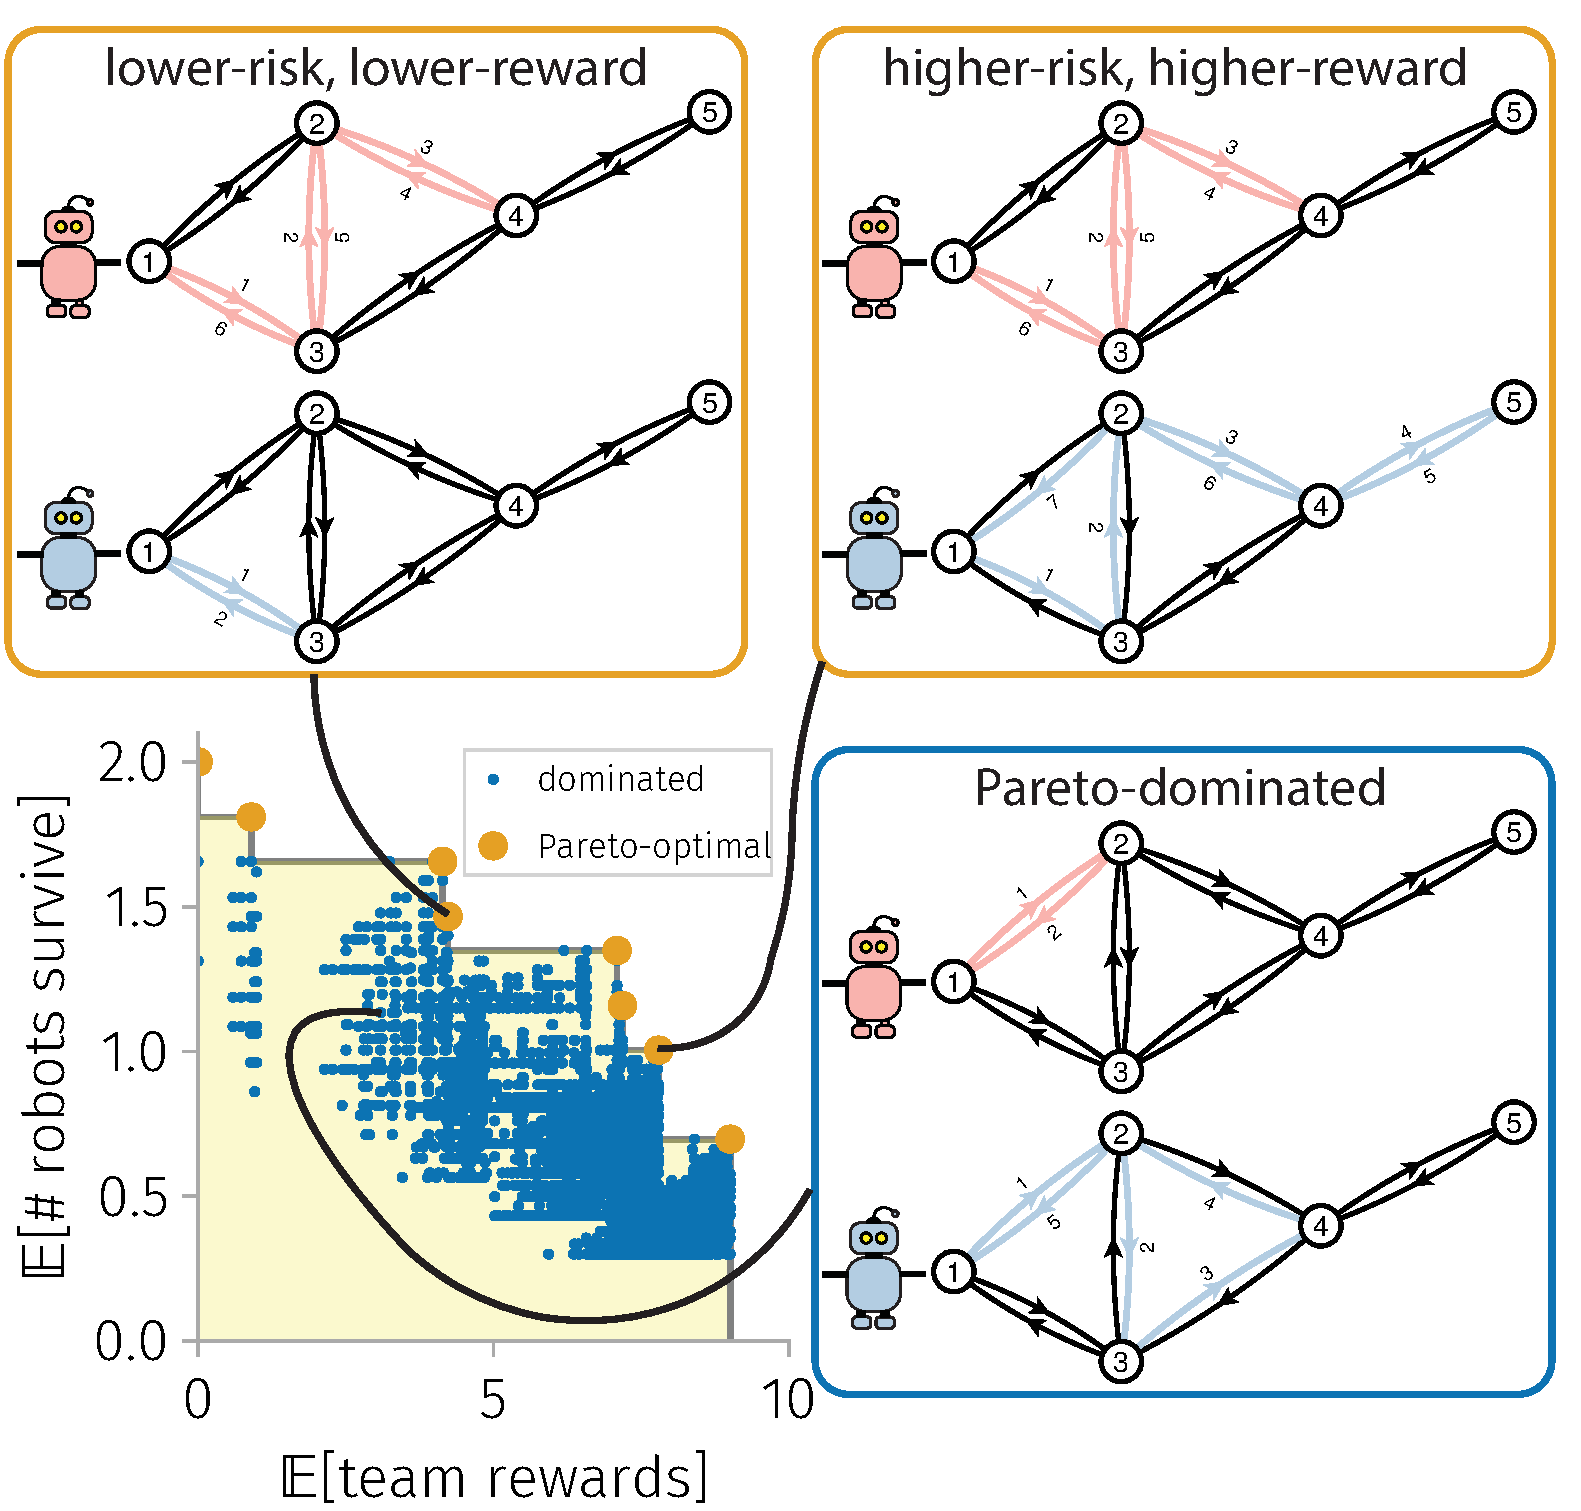
\includegraphics[width=\textwidth]{toy_pareto_front2.pdf}
	\caption{} \label{fig:pareto_optimal}
    \end{subfigure}
    \caption{
      The bi-objective team orienteering in hazardous environments (BOTOHE) problem.
      (a) A team of robots are mobile on a directed graph whose 
      nodes offer a reward to the team if visited by a robot and 
      arcs present a probability of destruction to robots that traverse them (tornado: 1/10 probability of destruction). The task is to plan the trails of the robots to maximize the expected reward collected and the expected number of robots that survive.
      (b) Pareto-optimal and -dominated robot-team trail plans scattered in objective space, with two Pareto-optimal plans and one Pareto-dominated plan shown.}
\end{figure}



\section{The bi-objective team orienteering in hazardous environments (BOTOHE) problem}
%In the risky team orienteering problem (RTOP), our task is to plan the trails of a team of mobile robots on a directed graph whose (i) nodes offer rewards to the team depending on the number of robots that visit them and (ii) edges, when traversed by a robot, impose a risk of robot failure/destruction.
%The trails are set at the beginning of the mission, then followed by the robots without updates during the mission---an offline setting. 
%For the bi-objective RTOP (BO-RTOP), we wish to find the set of Pareto-optimal trail plans for the robot team that maximize the expected (i) rewards collected by the team and (ii) the number of robots that survive the mission.

%A team of mobile robots must plan closed trails to follow on a directed graph, containing hazards, to collect rewards from nodes. The two conflicting objectives are to maximize the expected team-reward and number of robots that survive. We seek the Pareto-optimal set of robot-team trail plans.


\subsection{Problem setup}
Here, we frame the Bi-Objective robot-Team Orienteering in Hazardous Environments (BOTOHE) problem. 

A homogenous team of $K$ robots are mobile in an environment modeled as a directed graph $G=(\mathcal{V}, \mathcal{E})$. Each node $v \in \mathcal{V}$ represents a location in the environment (e.g., a room in a building). Each arc $(v, v^\prime) \in\mathcal{E}$, an ordered pair of distinct nodes, represents a one-way, direct spatial connection (e.g.\ a door- or hall-way) to travel from node $v$ to node $v^\prime$. 
\emph{Mobility} of the robots implies they may walk on the graph $G$, i.e. sequentially hop from a node $v$ to another node $v^\prime$ via traversing arc $(v, v^\prime)\in\mathcal{E}$.
All $K$ robots begin at a base node $v_b \in \mathcal{V}$. 
% TODO revisit
% We include one self-loop $(v_b, v_b) \in \mathcal{E}$ to allow the possibility for a robot to never leave the base node.
We assume $G$ is strongly connected so that each node is reachable.
% ---but, not necessarily complete. 

Owing to unpredictable and/or uncertain hazards in the environment, a robot incurs a probability of destruction of $1 - \omega(v, v^\prime)$ when, beginning at node $v$, it attempts to traverse arc $(v, v^\prime) \in \mathcal{E}$ to visit node $v^\prime$.
% following its trail $\rho$. 
Each outcome (survival or destruction) is an independent event. 
The arc survival probability map $\omega: \mathcal{E} \rightarrow (0, 1]$ is known, static over the course of the mission, and not necessarily symmetric (owing to e.g., [directional] air/water currents or sunlight or an adversary with limited attack range nearer one node than another).

%\vspace{-\baselineskip}
%\subparagraph{Interpretation.} 
%Each node $v\in \mathcal{V}$ represents a distinct location in the environment (e.g., a room in a building or a house in a neighborhood).
%Each arc $(v, v^\prime) \in \mathcal{E}$ represents a direct spatial connection (e.g., a doorway or a road) for traveling from location $v$ to location $v^\prime$.


% the best (e.g., shortest or safest) path (in Euclidean space) for a mobile robot to take from the location represented by node $v$ to the location represented by $v^\prime$.
% Note, we do not assume the graph is complete\footnote{i.e., not every pair of distinct nodes $\{v, v^\prime\}$ is joined by two edges $(v, v^\prime)$ and $(v^\prime, v)$. 
% e.g., consider a building with node $v$ representing a room on the first floor, node $v^\prime$ a room on the second floor, and node $u$ as the staircase between the first and second floors. Traveling from node $v$ to node $v^\prime$ necessitates passing through node $u$ first.}.

Each node $v\in \mathcal{V}$ of the graph $G$ offers a reward $r(v) \in  \mathbb{R}_{\geq 0}$ to the robot team if visited by one or more robots over the course of the mission.
The reward $r(v)$ quantifies the utility gained by the team when a robot e.g.\ delivers a resource to node $v$, takes an image of node $v$ and transmits it back to the command center, or actuates some process (e.g.\ turns a valve) at node $v$. 
The total reward collected by the team is additive among nodes of the graph. % The first objective of the BOTOHE is to maximize the team reward.
Note, 
(1) even if a robot is destroyed after leaving a node, the harvested reward from that node is still accumulated by the team; and
(2) multiple visits to a node by the same or distinct robot(s) do not give marginal reward over a single visit. % I.e.\ the reward from a node is irrevocably collected by the team [only] by the first robot to visit it.
%; and
%(3) the reward offered by a node could be negative, i.e. there could be a penalty to visit a node instead of an incentive.



%\paragraph{The probabilistic model of robot destruction during trail-following.} 

% The second objective of the BOTOHE is to maximize the number of robots that s.

%Thus, from the function  that assigns robot survival probabilities to each arc of the graph $G$, we can compute the survival probabilities of the $K$ robots following any given set of trails.
% plans $\{\rho_1, ..., \rho_K\}$.% and (2) the expected utility of the rewards harvested by the robots along their paths, which we write next. 



%\vspace{-\baselineskip}
%\subparagraph{Interpretation.} The hazards in the environment could originate from obstacles the robot could crash into, rough terrain or seas, severe weather, mines, corrosive chemicals, or adversaries capable of attacking the robots at the arcs and/or nodes.
%The stochasticity of the survival of a robot traversing an arc originates from e.g. (i) the unpredictability of an aerial robot crashing into an obstacle, a ground robot falling over rocks, or a surface aquatic robot succumbing to ocean waves, or (ii) adversaries with (a) an imperfect capability to detect and attack robots and/or (b) uncertain presence in the environment.

%\vspace{-\baselineskip}
%\subparagraph{Possible asymmetry.} We do not assume $\omega$ is symmetric, i.e., that $\omega(v, v^\prime) = \omega(v^\prime, v)$. The traversal from node $v$ to $v^\prime$ may be more dangerous than from $v^\prime$ to $v$ owing to e.g., (i) strong air or water currents in the direction $v^\prime$ to $v$ (asymmetric arc traversal) or (ii) an adversary with attack capability at node $v^\prime$ but not at $v$ (asymmetric dangers at nodes). %Even if edge traversal risks are symmetric, the action of visiting a node be risky, and node $v$ may be more or less dangerous than node $v^\prime$, breaking symmetry. 

% \paragraph{The robot-team trail plan.}
To collect rewards in this hazardous environment, the team of robots must plan a set\footnote{Since the robot team is homogenous, we consider the team trail plan as permutation-invariant and thus treat it as a set not a list.} of closed, directed trails $\mathcal{P}:=\{\rho_1, ..., \rho_K\}$ on the graph $G$ to follow.
% obot $k$ on the team plans to execute/follow a closed, directed trail $\rho_k$ on the graph $G$.  
% The set\footnote{Since the robot team is homogenous, we consider the optimal trail plans for the robots as permutation-invariant and thus track it as a set not a list.} of closed, directed trails $\mathcal{P}:=\{\rho_1, ..., \rho_K\}$ the robot-team plans to follow constitute the \emph{robot team trail plan} for the mission. 
A \emph{directed trail} \cite{clark1991first,graphtheory2} is an ordered list of nodes $\rho = (\rho[0], \rho[1], ..., \rho[\lvert \rho \rvert])$ where
(i) $\rho[i] \in \mathcal{V}$ is the $i$th node in the trail,  
(ii) for each node in the trail except the last, an arc joints it to the subsequent node, i.e., $(\rho[i-1], \rho[i])\in\mathcal{E}$ for $1 \leq i  \leq \lvert \rho \rvert$,
(iii) $\lvert \rho \rvert$ is the number of arcs traversed in the trail,
and
(iv) the arcs traversed in the trail are unique, i.e. each arc in the multiset $\{(\rho[i-1], \rho[i])\}_{i=1}^{\lvert \rho \rvert}$ has a multiplicity of one.
Note, unlike a path, the nodes in a trail are not necessarily distinct \cite{wilson1979introduction}.
A \emph{closed} trail begins and ends at the same node, i.e. $\rho [0]=\rho[\lvert \rho \rvert]$, which, here, $=v_b$.
Each trail $\rho_k$ belonging to the robot-team trail plan $\mathcal{P}$ constitutes a \emph{plan} because robot $k$ may be destroyed in the process of following $\rho_k$ and thus not \emph{actually} visit all nodes in $\rho_k$. A robot \emph{survives} the mission if it visits all nodes in its planned trail and returns to the base node. I.e., robot $k$ survives the mission if and only if it survived each edge traversal in its trail plan $\rho_k$.
%\vspace{-\baselineskip}
%\subparagraph{The static/offline setting.} 
%The robot-team trail plan $\mathcal{P}$ are set at the beginning of the mission, then followed by the robots without adaptation or updates during the mission in response to observing robot failure(s).
%i.e., robots cannot communicate their survival status to the command center during the mission and/or the command center cannot send updated instructions to the robots after the mission executes.

We wish to design the robot-team trail plan $\mathcal{P}$ to maximize two objectives: 
(1) the expected team \underline{r}eward, $\mathbb{E}[R]$, and (2) the expected number of robots that \underline{s}urvive the mission, $\mathbb{E}[S]$. Both $R$ and $S$ (i) are random variables owing to the stochasticity of robot survival while trail-following and (ii) depend on the robot-team trail plan $\mathcal{P}$ owing to different rewards among nodes and different dangers among arcs.
That is, the BOTOHE problem is:
\begin{equation}
	\max_{\mathcal{P}=\{\rho_1, ..., \rho_K\}} \left( \mathbb{E}[R(\mathcal{P})], \mathbb{E}[S(\mathcal{P})] \right)
	\label{eq:the_two_objs}
\end{equation}
when given the directed graph $G$ as a spatial abstraction of the environment, 
the homogenous team of $K$ mobile robots starting at the base node $v_b$,
the node reward map $r: \mathcal{V} \rightarrow \mathbb{R}_{\geq 0}$, and the arc survival probability map $\omega : \mathcal{E} \rightarrow (0, 1]$.
% the BOTOHE problem is to determine the optimal robot-team [closed] trail plan $\mathcal{P}$ that maximizes two-objectives, (1) the expected team-reward and (2) the expected number of robots that survive the mission:

Because the bi-objective optimization problem in eqn.~\ref{eq:the_two_objs} presents a conflict between designing the robot-team trail plan to maximize the expected reward \emph{and} the expected number of surviving robots, we seek the \emph{Pareto-optimal set} \cite{pardalos2017non,branke2008multiobjective} of team-robot trail plans. 
The conflict is: 
(1) to maximize survival, a risk-averse robot team would not visit a dangerous region even if large rewards were contained therein, sacrificing reward for survival; 
(2) to maximize reward, a daring robot team would visit a dangerous region even if only small rewards were contained therein, sacrificing survival for reward. 
Hence, a utopian robot-team trail plan that simultaneously maximizes \emph{both} reward and survival objectives is unlikely to exist; the ultimate team trail plan selected for the mission must strike some tradeoff between reward and survival.
By definition, a \emph{Pareto-optimal} \cite{pardalos2017non,branke2008multiobjective} robot-team trail plan $\mathcal{P}^*$ cannot be altered to increase the survival objective $\mathbb{E}[S(\mathcal{P}^*)]$ without compromising (decreasing) the reward objective $\mathbb{E}[R(\mathcal{P}^*)]$---and vice versa. See Fig.~\ref{fig:pareto_optimal} and the formal definition below.
The Pareto-optimal set of team trail plans is valuable for presenting a \emph{portfolio} of team trail plans to a human decision-maker, who then (a) examines the possible tradeoffs then (b) ultimately, invokes their values on team-reward vs.\  robot-survival by selecting a reasonable robot-team trail plan from the Pareto set to execute.



% TODO say later somehwere: For the reward objective, the daring robots \emph{all} plan to enter dangerous regions---regardless of the potential reward; such node-visitation redundancy endows the team reward with robustness to robot failures. 


%\vspace{-\baselineskip}
%\subparagraph{Objective \#1: the expected reward collected by the robots.}
%Let $T_v(\mathcal{P}) $ be the number of robots on the team with trail plans $\mathcal{P}$ that ultimately visit node $v$.
%Because of the stochasticity of robot survival while trail-following, and thus of which nodes in the trail plan each robots ultimately visits, $T_v$ is a random variable.
%Then, the total team \underline{r}ewards collected by the robot-team following trail plans $\mathcal{P}$ is also a random variable:
%\begin{equation}
%R(\mathcal{P}) = \sum_{v\in\mathcal{V}} r_v\left ( T_v(\mathcal{P}) \right)
%\end{equation}
%that sums the rewards received from each node of the graph $G$.
%
%\vspace{-\baselineskip}
%\subparagraph{Objective \#2: the expected number of robots that survive the mission.}
%Let $S(\mathcal{P})$ be the number of robots, on a robot team with trail plans $\mathcal{P}$, that ultimately \underline{s}urvive the mission. Because of the stochasticity of robot survival while trail-following, $S$ is a random variable. 
%
%We wish to devise robot-team trail plans $\mathcal{P}$ to maximize both (1) the expected team reward, $\mathbb{E}[R(\mathcal{P})]]$, and (2) the expected number of robots that survive the mission, $\mathbb{E}[S(\mathcal{P})] \in (0, K]$. We derive formulas for the values of the two objectives in terms of the robot-team trail plans later (see eqns.~\ref{eq:formula_obj1} and \ref{eq:formula_obj2}). 



%, and (iv) do not assume the team reward viewed as a function over the set of visited nodes is monotone because we allow for negative rewards.
% {\color{red} k then make this happen in example, and how then does $\eta_r$ work if it can be negative? }



%Given the conflict between the two objectives, 

% A human decision-maker must invoke their values to make this tradeoff.% and determine if robots should plan to enter dangerous regions to attempt collection of large rewards there. 


\paragraph{Formal definition of Pareto-optimality and Pareto-front.}
Plan $\mathcal{P}^*$ belongs to the Pareto-optimal set of plans if and only if no other plan $\mathcal{P}^\prime$ \emph{Pareto-dominates} it. By definition, a plan $\mathcal{P}^\prime$ Pareto-dominates plan $\mathcal{P}^*$ if and only if both:
\begin{align}
	\left (\mathbb{E}[R(\mathcal{P}^\prime)] \geq \mathbb{E}[R(\mathcal{P}^*)]  \right) & \wedge \left( \mathbb{E}[S(\mathcal{P}^\prime)] \geq \mathbb{E}[S(\mathcal{P}^*)] \right) \\
	\left( \mathbb{E}[R(\mathcal{P}^\prime)] > \mathbb{E}[R(\mathcal{P}^*)] \right) & \vee \left( \mathbb{E}[S(\mathcal{P}^\prime)] > \mathbb{E}[S(\mathcal{P}^*)] \right).
\end{align}
So, a Pareto-dominating plan $\mathcal{P}^\prime$ is not worse than a Pareto-dominated plan $\mathcal{P}^*$ for reward nor for survivability and is better for one or both of them.
If a plan $\mathcal{P}^\prime$ were to Pareto-dominate another plan $\mathcal{P}^*$, one would objectively never choose plan $\mathcal{P}^*$ over plan $\mathcal{P}^\prime$, regardless of the values they place on the two objectives. The \emph{Pareto front} is the set of objective vectors $\{(\mathbb{E}[R(\mathcal{P}^*)], \mathbb{E}[S(\mathcal{P}^*)])\}$ associated with the Pareto-optimal set of team trail plans $\{\mathcal{P}^*\}$.  

\paragraph{Comparison with TSOP.}
The BOTOHE problem formulation follows the offline TSOP \cite{jorgensen2018team} with three modifications: we 
(i) omit the constraints that each robot survives above a threshold probability (e.g., we accept if one [un-crewed] robot bears much more risk of destruction than another during the mission),
(ii) allow robots to follow trails instead of restricting to paths, as paths prevent robots from visiting a given node more than once and thus from e.g., harvesting reward from a leaf node having one in-degree and one out-degree involving the same node, 
and
(iii) specify two objectives instead of one and seek the Pareto-optimal set of team trail plans to examine trade-offs between reward and survival before selecting a team trail plan.

\subsection{Probability distributions and expectations of $R(\mathcal{P})$ and $S(\mathcal{P})$}
We now write formulas for the two objectives---the expectations of the team reward $R(\mathcal{P})$ and of number of robots that survive the mission $S(\mathcal{P})$---as a function of the robot-team trail plan $\mathcal{P}$. 
These formulas follow from the directed graph $G$, arc survival probability map $\omega$, and node reward map $r$. Fig.~\ref{fig:notation} illustrates our notation.
% Given a proposed robot-team trail plan $\mathcal{P}$, we can calculate the two objectives $\mathbb{E}[R(\mathcal{P})]$ and $\mathbb{E}[S(\mathcal{P})]$ via eqns.~\ref{eq:formula_obj1} and \ref{eq:formula_obj2}, respectively.

\begin{figure}[h!]
    \centering
    	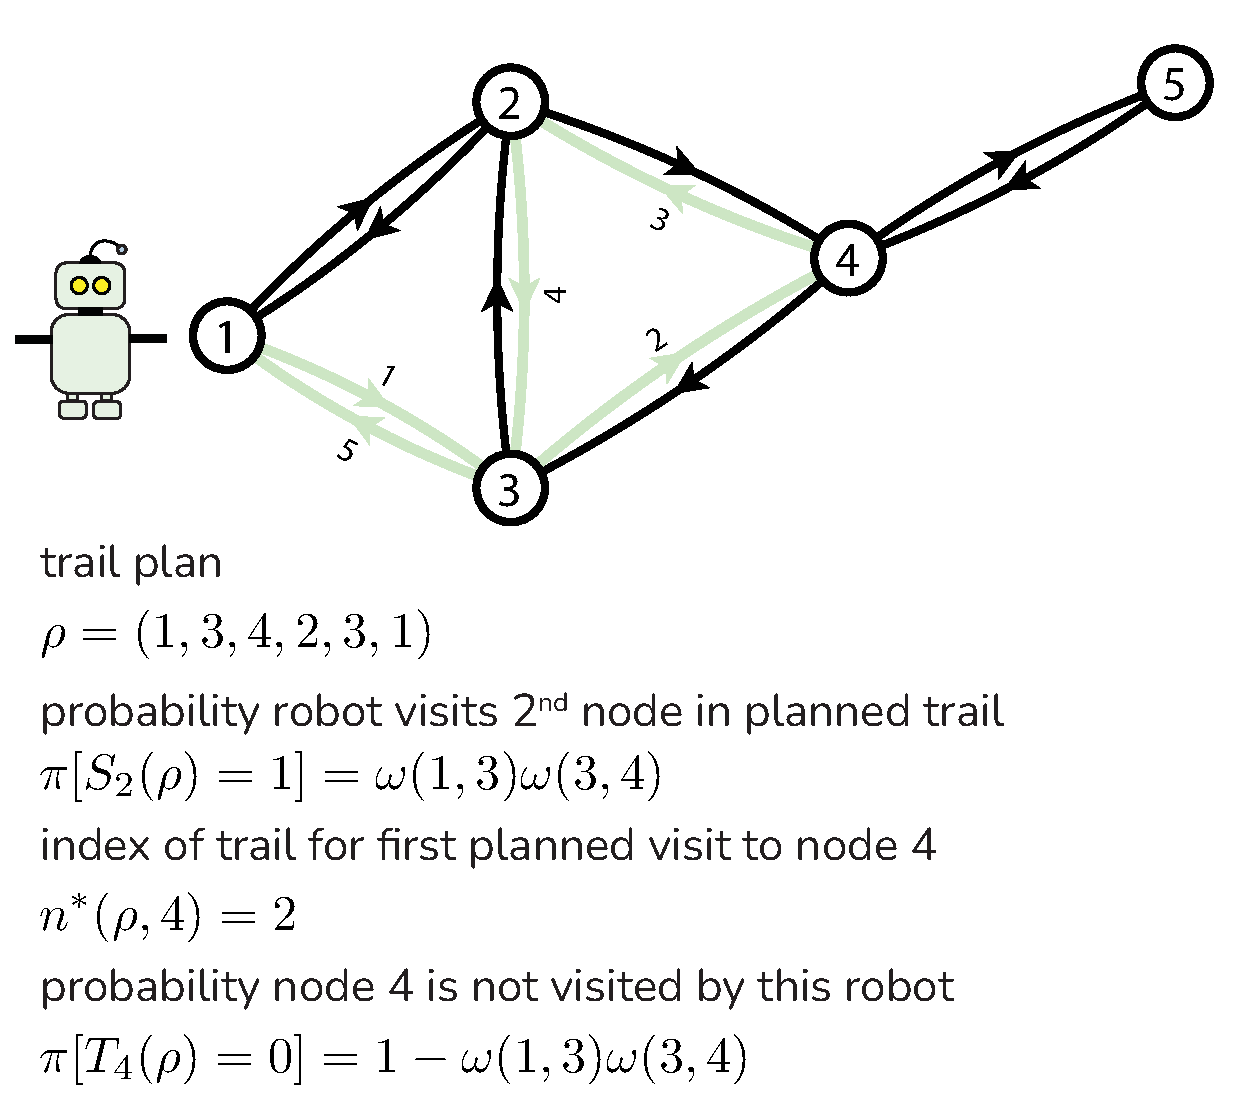
\includegraphics[width=0.6\textwidth]{notation.pdf}
    \caption{Illustrating notation for a particular robot's trail plan.} \label{fig:notation}
\end{figure}

\subsubsection{The survival of a single robot along its followed trail}
Central to computing both $\mathbb{E}[S(\mathcal{P})]$ and $\mathbb{E}[R(\mathcal{P})]$ is the probability that a robot survives to reach a given node in its planned trail.
Let $S_n(\rho)$ for $0 \leq n \leq \lvert \rho \rvert$ be the Bernoulli random variable that is one if a robot following trail $\rho$ survives to visit the $n$th node in the trail and zero otherwise. 
For the event of survival, the robot must survive traversal of \emph{all} of the first $n$ arcs in its trail to visit node $\rho[n]$. More, the survival of a robot over each arc traversal attempt is an independent event. Therefore, the probability that a robot following trail $\rho$ successfully visits node $\rho[n]$ is the product of the survival probabilities of the first $n$ arc-hops in the trail:
\begin{equation}
	\pi[S_n(\rho) = 1] = \prod_{i=1}^n \omega(\rho[i-1], \rho[i]) 
	% \text{ for } 0 \leq n \leq \lvert \rho \rvert \\%\in \{1, ..., \lvert \rho \rvert\} 
	= 1 - \pi[S_n(\rho) = 0]. \label{eq:pi_S_n}
\end{equation} %The factorization owes to the independence of the arc-traversal$+$node-visit survival events.
The second equality follows because the complement of the event of survival is destruction.

\subsubsection{Expected number of robots that survive}
Now, we write a formula for the expected number of robots that survive the mission, $\mathbb{E}[S(\mathcal{P})]$. The event of survival of each robot is independent of the other robots.
Consequently, the number of robots that survive the mission, $S$, is the sum of the Bernoulli random variables indicating the survival of each robot over its entire planned trail:
\begin{equation}
	S(\mathcal{P}=\{\rho_1, ..., \rho_K\})=\sum_{k=1}^K S_{\lvert \rho_k \rvert}(\rho_k). \label{eq:R_sum}
\end{equation}
Thus, $S$ follows the Poisson-Binomial distribution \cite{tang2023poisson}.
%Specifically, the probability that $s$ robots survive the mission is:
%\begin{multline}
%	\pi[S(\mathcal{P})=s] = \sum_{\substack{\mathcal{R} \subseteq \{1, ..., K\}  \\ \lvert \mathcal{R} \rvert = s} } \,
%	\prod_{k \in \mathcal{R}} \pi[S_{\lvert \rho_k \rvert}(\rho_k) = 1]
%	\prod_{k^\prime \in \{1, ..., K\} \setminus \mathcal{R}}
%	 \pi[S_{\lvert \rho_{k^\prime} \rvert}(\rho_{k^\prime}) = 0]
%	 , \\ \text{ for } 0 \leq s \leq K.
%	\label{eq:R_pb}
%\end{multline}
%Eqn.~\ref{eq:R_pb} sums over all $\binom{K}{s}$ possible size-$s$ surviving subsets $\mathcal{R}$ of the $K$ robots. The first product is the probability that all of those robots in $\mathcal{R}$ indeed survive their closed trails. The second product is the probability that the other robots outside of $\mathcal{R}$ indeed get destroyed somewhere along their closed trails.
Seen from eqn.~\ref{eq:R_sum} and the linearity of the expectation operator, the expected number of robots that survive the mission is:
\begin{equation}
	\mathbb{E}[S(\mathcal{P}=\{\rho_1, ..., \rho_K\})]=\sum_{k=1}^K \mathbb{E}[S_{\lvert \rho_k \rvert}(\rho_k)] = \sum_{k=1}^K  \pi[S_{\lvert \rho_k \rvert}(\rho_k) = 1] \label{eq:formula_obj2}
\end{equation} with $\pi[S_{\lvert \rho_k \rvert}(\rho_k) = 1]$ given in eqn.~\ref{eq:pi_S_n}.

\subsubsection{Expected team reward}
Now, we write a formula for the expected team reward, $\mathbb{E}[R(\mathcal{P})]$. 
% Obviously, the outcome $S_n(\rho)=0$ implies $S_{n+i}(\rho)=0$ for $1 \leq i \leq \lvert \rho \rvert-n$ since, once a robot is destroyed at some node/arc along its trail, it cannot visit subsequent nodes in the planned trail.

First, we calculate the probability that a robot following a given trail $\rho$ does not visit a given node $v\in \mathcal{V}$.
Let the Bernoulli random variable $T_v(\rho)$ be one if a robot following trail $\rho$ visits node $v$ and zero if it does not.
If node $v$ is not in the planned trail $\rho$, $T_v(\rho)=0$ with certainty. 
Now, suppose node $v$ is in the planned trail $\rho$. Let $n^*$ be the index in the trail where the robot plans its first visit to node $v$:
\begin{equation}
n^*(\rho, v) = \min_{
	\substack{n \in \{0, ..., \lvert \rho \rvert\} \\ \rho[n] = v}
} n.
\end{equation}
Then, $T_v(\rho)=S_{n^*}(\rho)$ because the robot visits node $v$ if and only if it survives its first $n^*$ arc-hops to first land on node $v$ in the trail. 
So, the probability node $v$ is not visited by a robot following trail $\rho$ is:
\begin{equation}
	\pi[T_v(\rho) = 0] = 
	\begin{cases}
		1 & v\notin \rho\\
		 \pi [S_{n^*(\rho, v)}(\rho)=0 ] & v \in \rho
	\end{cases}
	 \label{eq:pi_T_v}
\end{equation}
with $\pi[S_{n^*}(\rho)=0]$ calculated using eqn.~\ref{eq:pi_S_n}.

Second, we calculate the probability that a given node $v\in\mathcal{V}$ is visited by one or more robots on a team following trail plans $\mathcal{P}=\{\rho_1, ..., \rho_K\}$. Only in this event is the reward offered by that node, $r(v)$, accumulated by the team.
Let $T_v(\mathcal{P})$ be the Bernoulli random variable that is one if one or more robots on the team with trail plans $\mathcal{P}$ visit node $v$ and zero otherwise (i.e.\ if and only if zero of the robots visit $v$).
The complement of the event $T_v(\mathcal{P})=1$ is that all $K$ robots do not visit node $v$ (independent events), so:
\begin{equation}
	\pi [T_v( \{\rho_1, ..., \rho_K\} ) = 1] = 
	1 - \prod_{k=1}^K \pi[T_v(\rho_k)=0].
	\label{eq:pi_T_v_all}
\end{equation} 
with $\pi[T_v(\rho) = 0]$ in eqn.~\ref{eq:pi_T_v}.

Finally, the total team reward collected by the robot-team following trail plan $\{\rho_1, ..., \rho_K\}$ is the sum of the rewards given to the team by each node:
\begin{equation}
R(\{\rho_1,...,\rho_K\}) = \sum_{v\in\mathcal{V}} r(v)  T_v(\{\rho_1, ..., \rho_K\}),
\end{equation} where the reward from node $v$, $r(v)$, is accumulated if and only if node $v$ is visited by one or more robots (i.e. iff $T_v(\mathcal{P})=1$).
So, the expected reward accumulated over the mission by a robot-team following trail plans $\{\rho_1, ..., \rho_K\}$ is:
\begin{equation}
	\mathbb{E}[R(\{\rho_1,...,\rho_K\})]= \sum_{v\in\mathcal{V}} r(v) \pi[T_v(\{\rho_1, ..., \rho_K\}) = 1] \label{eq:formula_obj1}
\end{equation}
with $ \pi[T_v(\{\rho_1, ..., \rho_K\}) = 1]$ given in eqn.~\ref{eq:pi_T_v_all}.

\subsubsection{Summary: computing the objective values associated with a robot-team trail plan}
Given a robot-team trail plan $\mathcal{P}:=\{\rho_1,...,\rho_K\}$, we can compute the expected team reward, $\mathbb{E}[R(\mathcal{P})]$, via eqn.~\ref{eq:formula_obj1} and the expected number of robots that survive the mission, $\mathbb{E}[S(\mathcal{P})]$, via eqn.~\ref{eq:formula_obj2}.


% harvest risk different from visit risk. once harvested, then no longer risk for other robots to visit that node.

\section{Bi-objective ant colony optimization to search for the Pareto-optimal robot-team trail plans}
To efficiently search for the Pareto-optimal set of robot-team trail plans defined by eqn.~\ref{eq:the_two_objs}, we employ bi-objective (BO) ant colony optimization (ACO) \cite{iredi2001bi}. ACO \cite{dorigo2006ant,bonabeau1999swarm,blum2005ant,simon2013evolutionary} is a meta-heuristic for combinatorial optimization problems that can be framed as a search for optimal paths or trails on a graph. As a swarm intelligence method \cite{bonabeau1999swarm}, 
ACO is inspired by the behavior of ants efficiently foraging for food via laying and following pheromone trails \cite{bonabeau2000inspiration}. See Box~\ref{box:ants}. 
Variants of the single-robot- and team-orienteering problem have been efficiently and effectively solved by ACO \cite{ke2008ants,chen2015multiobjective,verbeeck2017time,sohrabi2021acs,chen2022environment,montemanni2011enhanced} (as well as by other [meta-]heuristics \cite{gavalas2014survey,dang2013effective,chao1996fast,butt1994heuristic}), but not the TSOP.

\begin{mybox}[label=box:ants, breakable]{Pheromone trail laying and following by foraging ants}
Advantageously \cite{deneubourg1983probabilistic}, a foraging ant colony can (well, for some ant species) collectively select 
(i) the shortest path from its nest to a food source \cite{goss1989self}
and
(ii) the highest quality food source among multiple options equidistant from its nest \cite{beckers1993modulation}. 
Largely, but not exclusively \cite{evison2008combined,czaczkes2015trail,robinson2005no}, this self-organizing of the colony is mediated by individual ants laying and following pheromone trails \cite{czaczkes2015trail}.

Pheromone is a relatively volatile chemical \cite{david2009trail} that an ant can both secrete and receive as an olfactory cue \cite{knaden2016sensory}. Thereby, pheromone allows for \emph{indirect} communication between ants in the colony. 
On its way back to the nest from a food source, an ant deposits pheromone on the ground in proportion to the quality of the food source \cite{beckers1993modulation}.
Shorter paths to higher quality food sources accumulate pheromone from ants more quickly.
Since ants are recruited to and follow pheromone \cite{beckers1993modulation,czaczkes2015trail}, these paths recruit more ants and get reinforced. Via this positive feedback mechanism, the colony can collectively select the shortest paths from the nest to the highest-quality food sources \cite{jackson2006communication,czaczkes2015trail,bonabeau1999swarm}.
The pheromone trails laid by the colony form a \emph{collective memory}, locally guiding ants to high-quality food sources and short paths to them \cite{jackson2006communication}.
Some species of ants can deposit multiple species of pheromone (from different glands) with e.g.\ different longevities \cite{czaczkes2015trail}, allowing for more complex indirect communication \cite{jackson2006communication,robinson2005no}.

As negative feedback mechanisms, 
(i) pheromone evaporates over time \cite{jackson2006communication,david2009trail,van2011temperature}, allowing the ant colony to ``forget'' trails to exhausted food sources,
and 
(ii) ants deposit less pheromone on trails (a) with already-high pheromone concentrations \cite{czaczkes2013ant} or (b) leading to food sources already occupied by their nestmates \cite{wendt2020negative}.

Ants select among pheromone trails with some degree of stochasticity \cite{deneubourg1990self}, which is beneficial for 
(i) continual exploration to find even shorter paths and even higher-quality food sources, 
(ii) exploiting multiple food sources in parallel, 
and 
(iii) plasticity in a dynamic environment \cite{deneubourg1983probabilistic,shiraishi2019diverse,deneubourg1986random,dussutour2009noise,edelstein1995trail}.


In summary, a colony of decentralized ants laying and following pheromone trails can exhibit complex, self-organizing behavior.
The pheromone trails serve as a form of collective memory and a means for indirect communication.
Loosely, ants can solve optimization problems through combining positive feedback (reinforcing good paths), negative feedback (pheromone evaporation), and randomness (exploring new paths). \cite{bonabeau1997self,bonabeau1999swarm,goss1989self,jackson2006communication,edelstein1995trail,watmough1995modelling}.
\end{mybox}

In bi-objective ACO \cite{iredi2001bi}, we simulate a heterogenous colony of artificial ants walking on the graph $G$ and, by loose analogy, foraging for food over many iterations. 
At each iteration, each worker ant stochastically constructs a robot-team trail plan $\{\rho_1, ..., \rho_K\}$ robot-by-robot, arc-by-arc, biased by 
(i) the amounts of two species of pheromone on the arcs that encode the colony's memory of trails that gave high reward and high survival
and 
(ii) two heuristics that score the greedy, \emph{a priori} appeal of each arc for constructing trails that give high reward and high survival.  
As a division of labor, each worker ant specializes by searching for team trail plans belonging to a different region of the Pareto-front.
At the end of each iteration, ants that found Pareto-optimal team trail plans over that iteration deposit reward and survival pheromone on the arcs involved, in proportion to the expected reward and survival, respectively, achieved by the plan.
An elitist ant \cite{dorigo1996ant} maintains a set of global (i.e, over all iterations) Pareto-optimal team trail plans and also deposits pheromone on arcs.
Finally, to prevent stagnation and promote continual exploration, a fraction of the pheromone evaporates each iteration. After many iterations, the ACO algorithm returns the [approximate\footnote{The ACO meta-heuristic is not guaranteed to find all of the Pareto-optimal solutions nor neglect to include a Pareto-dominated solution.}] Pareto-optimal set of robot-team trail plans maintained by the elitist ant. 


\subsection{The heterogenous artificial colony of ants, the pheromone, and the heuristics}
Our heterogenous artificial ant colony consists of (i) $N_{\text{ants}}$ worker ants and (ii) an elitist ant.
Worker ant $i\in\{1, ..., N_{\text{ants}}\}$ in the colony is assigned a parameter $\lambda_i := (i-1) / (N_{\text{ants}}-1)$ dictating its balance of the two objectives when searching for Pareto-optimal team trail plans.
A $\lambda$ closer to zero (one) implies the ant prioritizes maximizing the expected reward $\mathbb{E}[R]$ (robot survivals $\mathbb{E}[S]$). 
So, different ants seek team trail plans belonging to different regions of the Pareto front.
The elitist ant maintains the global-Pareto-optimal set of team trail plans.

% \subsection{Pheromone levels and heuristic scores on the arcs of the graph}
Each arc $(v, v^\prime)\in\mathcal{E}$ of the graph is associated with 
(i) amounts of two distinct species of pheromone, reward pheromone $\tau_R(v, v^\prime)$ and survival pheromone $\tau_S(v, v^\prime)$, and 
(ii) two heuristic scores $\eta_R(v, v^\prime)$ and $\eta_S(v, v^\prime)$.
Both $\tau_{R, S}(v, v^\prime)>0$ and $\eta_{R, S}(v, v^\prime)>0$ score the promise of arc $(v, v^\prime)$ for belonging to Pareto-optimal team trail plans that maximize $\mathbb{E}[R, S]$ and guide worker ants' construction of robot-team trail plans.
The pheromone is (1) learned, reflecting the past collective experience/memory of the ant colony, and (2) dynamic over iterations, due to deposition by the ants and evaporation.
By contrast, the heuristic is static and scores the \emph{a priori}, greedy/myopic appeal of each arc.
We incorporate the heuristics into ACO to accelerate its convergence.
%
%
%The ants lay and [probabilistically] follow two distinct species of artificial pheromone on the arcs of the graph $G$---one species associated with each objective. 
%
%The pheromone maps $\tau_R:\mathcal{E}\rightarrow \mathbb{R}_+$ and $\tau_S:\mathcal{E}\rightarrow \mathbb{R}_+$ give the amount of reward and survivability pheromone, respectively, on each arc of $G$.
%The value $\tau_R(v, v^\prime)$ ($\tau_S(v, v^\prime)$) scores the promise of arc $(v, v^\prime)$, learned from all past experience of the ant colony, for belonging to Pareto-optimal team trail plans that maximize the expected reward $\mathbb{E}[R]$ (number of robots that survive $\mathbb{E}[S]$).
%As opposed to being static, the pheromone maps $\tau_{R,S}$ change from iteration-to-iteration due to deposition by the ants and evaporation. 
% Together, the pheromone maps $\tau_{R,S}$ represent a [fading] memory of the artificial ant colony about the propensity of each arc to belong to Pareto-optimal robot-team trail plan and, vaguely, where along the Pareto-front the plan might li.e.
% vaguely, through laying and following \emph{two} species of pheromone, .

\subsection{Constructing robot-team trail plans}
Each iteration, every worker ant stochastically constructs a team trail plan $\mathcal{P}=\{\rho_1, ..., \rho_K\}$ by sequentially allocating trails to the robots while [conceptually] following the closed trail the ant designs for each robot. Computing the objectives achieved under each plan made by each ant, via eqns.~\ref{eq:formula_obj2} and \ref{eq:formula_obj1}, gives the colony data $\{ (\mathcal{P}_i, \mathbb{E}[R(\mathcal{P}_i)], \mathbb{E}[S(\mathcal{P}_i)])\}_{i=1}^{N_{\text{ants}}}$. This data is used by the worker ants to deposit pheromone on the arcs and by the elitist ant to update the global Pareto-optimal set.
% It assigns trails to the robots sequentially, robot-by-robot. 
% i.e. fully constructs the closed trail for robot 1, $\rho_1$, then $\rho_2$ for robot 2, and so on, up to robot $K$.
% For each robot trail it constructs, the ant starts at the base node $v_b$, then, arc-hop by arc-hop, constructs the closed trail on the graph that the robot will follow. 

A worker ant constructs a robot trail by iteratively applying a stochastic, partial-trail extension rule until the closed trail is complete. Suppose an ant with objective-balancing parameter $\lambda$ is constructing the closed trail for robot $k$, $\rho_k$, and currently resides at node $v=\rho_k[i]$.
Namely, the ant has selected (i) the trails for the previous $k-1$ robots, $(\rho_1, ..., \rho_{k-1})$, and (ii) an incomplete/partial trail for robot $k$, $\tilde{\rho_k}=(v_b, \rho_k[1], ..., \rho_k[i]=v)$, giving its first $i$ arc-hops.
The ant extends the partial trail $\tilde{\rho_k}$ for robot $k$ by choosing the next node $\rho_k[i+1]$  
via a roulette-wheel selection of outgoing arcs of $v$ not yet traversed in $\tilde{\rho_k}$.
Specifically, the probability of next hopping to node $v^\prime$ across arc $(v, v^\prime)\in\mathcal{E}$ not yet traversed in the partial trail $\tilde{\rho_k}$ is:
 \begin{equation}
	\pi(v^\prime \mid \rho_1, ..., \rho_{k-1}, \tilde{\rho_k}) \propto 
		 \left[\tau_R(v, v^\prime) \eta_R(v, v^\prime; \rho_1, ..., \rho_{k-1},\tilde{\rho_k}) \right]^{1-\lambda} \left[ \tau_S(v, v^\prime) \eta_S(v, v^\prime) \right]^\lambda.
	 \label{eq:prob_x_y}
\end{equation}
The partial trail is more likely to be extended with $v^\prime=:\rho_k[i+1]$ if arc $(v, v^\prime)$ has more pheromone $\tau_{R, S}(v, v^\prime)$ and/or greedy heuristic appeal $\eta_{R, S}(v, v^\prime)$---with more or less emphasis on the reward or survivability pheromone/heuristic depending on the ant's $\lambda$.
Note, the probability of transitioning to a node $v^\prime$ is zero if $(v, v^\prime) \notin \mathcal{E}$ or if arc $(v, v^\prime) \in \mathcal{E}$ was already traversed in the partial trail $\tilde{\rho_k}$.
Iteratively extending the partial trail using eqn.~\ref{eq:prob_x_y}, the ant completes the trail for robot $k$ after it traverses the self-loop of the base node, $(v_b, v_b)$, signifying an end. Then, the ant begins trail construction for robot $k+1$ if $k<K$ or completes its team trail plan $\mathcal{P}$ if $k=K$. 


% While the pheromone maps $\tau_{R,S}$ encode the ants colony's past experiences and are dynamic over iterations, the static, heuristic, experience-independent maps $\eta_{R,S}(v, v^\prime)$ score the [greedy] appeal, in terms of maximizing $\mathbb{E}[R]$ and $\mathbb{E}[S]$, respectively, of hopping from $v$ to $v^\prime$. 

\paragraph{Heuristics.} 
For the survivability objective, we score the desirability of arc $(v, v^\prime)$ with the probability of the robot surviving traversal of that arc, $\eta_S(v, v^\prime):=\omega(v, v^\prime)$. This survival heuristic is myopic because it does not consider survivability of arcs later in the trail. 
For the reward objective, we greedily score the desirability of arc $(v, v^\prime)$ with the expected marginal reward the team receives by robot $k$ visiting node $v^\prime$ next, which is $r(v^\prime)$ if 
(i) none of the previous $k-1$ robots visit node $v^\prime$, 
(ii) node $v^\prime$ is not planned to be visited earlier in the trail of robot $k$, and
(iii) robot $k$ survives its hop to node $v^\prime$
and zero otherwise:
% Consequently, $\eta_R$ considers both the previous $k-1$ robots' trails and robot $k$'s partial trail $\tilde{\rho_{k}}$:
\begin{equation}
	\eta_R(v, v^\prime; \rho_1, ..., \rho_{k-1}, \tilde{\rho_k}) :=  
	 \pi[ T_{v^\prime}(\{\rho_1, ..., \rho_{k-1}\}) = 0)] \mathcal{I}[v^\prime \notin \tilde{\rho_k}] \omega(v, v^\prime) r(v^\prime ) \label{eq:eta_R}
\end{equation}
with $\mathcal{I}(\cdot)$ the indicator function. This reward heuristic is myopic because it does not account for rewards robot $k$ could collect further along the trail nor the trails of the remaining robots on the team. 
% {\color{red} handle negative rewards?}
Note, to prevent either heuristic from being exactly zero (resulting in \emph{never} selecting that arc), we add a small number $\epsilon$ to each heuristic.


\subsection{Pheromone update}
At the end of each iteration, we update the pheromone maps $\tau_R$ and $\tau_S$ to capture the experience of the ants in finding Pareto-optimal robot-team trail plans, better-guide the ants' trail-building in the next iteration, and prevent stagnation (premature convergence). 


The pheromone update rule is:
\begin{equation}
	\tau_{R, S}(v, v^\prime) \leftarrow (1-\rho) \tau_{R,S}(v, v^\prime)  + \Delta \tau_{R,S}(v, v^\prime) \text{ for } (v, v^\prime) \in \mathcal{E}, \label{eq:tau_update}
\end{equation}
with $\rho \in (0, 1)$ the evaporation rate (a hyperparameter) and $\Delta \tau_{R,S}(v, v^\prime)$ the amount of new pheromone deposited on arc $(v, v^\prime)$ by the ants.

Evaporation, accomplished by the first term in eqn.~\ref{eq:tau_update}, removes a fraction of the pheromone on every arc. This negative feedback mechanism prevents premature convergence to suboptimal trails and encourages continual exploration.

Deposition, accomplished by the second term in eqn.~\ref{eq:tau_update}, constitutes indirect communication to ants in future iterations about which arcs tend to belong to Pareto-optimal team trail plans and the value of the expected reward and robot survivals achieved under those plans.
First, the ants \emph{collaborate} by 
(i) among the worker ants, comparing the solutions constructed \emph{this} iteration to obtain the \emph{iteration}-Pareto-optimal set of plans
and 
(ii) worker ants sharing the solutions constructed this iteration with the elitist ant, who then updates the \emph{global}-Pareto-optimal set.
Second, the worker ants with an iteration-Pareto-optimal team trail plan execute their constructed plan while depositing pheromone on the arcs.
Third, the elitist ant executes all global-Pareto-optimal team trail plans while depositing pheromone on the arcs. Each ant deposits both reward and survival pheromone in proportion to the reward and survival objectives, respectively, achieved under the plan they are following. (The value of the objective is analogous with food quality). 
Specifically, amalgamating the iteration- and global-Pareto-optimal team trail plans into a multiset $\{(\mathcal{P}_p^*, \mathbb{E}[R(\mathcal{P}_p^*)], \mathbb{E}[R(\mathcal{P}_p^*)])\}_{p=1}^P$, arc $(v, v^\prime)$ receives pheromone:
%Now, each time arc $(v, v^\prime)$ is traversed in trails of a [iteration- or global-]Pareto-optimal plan $\mathcal{P}^*_p$, 
%this [worker- or elitist-] ant deposits pheromone of each species on it in proportion to the objective achieved with $\mathcal{P}^*_p$:
\begin{equation}
	 \Delta \tau_{R,S}(v, v^\prime) := 
	\frac{1}{P} \sum_{p=1}^{P} \mathbb{E}[R(\mathcal{P}^*_p), S(\mathcal{P}^*_p)] 
	\kappa_{v, v^\prime}(\mathcal{P}^*_p) 
%	% sum over trails in the plan
%	\sum_{k=1}^K 
%	% sum over arcs in the trail
%	\sum_{i=1}^{\lvert \rho_k^{(p)}\rvert}
%	% indicator
%	\mathcal{I} \left[ 
%		(v, v^\prime)=(\rho_k^{(p)}[i-1], \rho_k^{(p)}[i])
%	\right].
\end{equation}
where $\kappa_{v, v^\prime}(\mathcal{P}^*_p)$ counts the number of times arc $(v, v^\prime) \in \mathcal{E}$ appears in team trail plan $\mathcal{P}^*_p$.
%The sums are over, left-to-right, Pareto-optimal plans, robot trails in those plans, and arcs in those robot trails. 
%The latter two sums count the number of times the arc $(v, v^\prime)$ appears in $\mathcal{P}^*_p$.
By construction, arcs that receive the most reward (survival) pheromone frequently belong to trails in the Pareto-optimal team trail plans with high reward (survival).

We initialize the pheromone maps as uniform: for each arc $(v, v^\prime)\in\mathcal{E}$, $\tau_s(v, v^\prime) := K$ and $\tau_r(v, v^\prime) := \sum_{v \in \mathcal{V}} r(v)$. 
First, compared to the amount of pheromone that could accumulate over iterations, this small quantity allows the heuristic to dominantly bias the beginning of the search.
Second, this initialization accommodates different numbers of robots and ranges of rewards for different problems.

\subsection{Shared versus per-robot pheromone maps}
The reward and survival pheromone maps are shared by the ant colony as a form of collective memory of arcs that led to Pareto-optimal trails with high expected reward and survival. Through sharing the two pheromone maps, the ants in the colony, despite focusing on different regions of the Pareto-front, collaborate in finding Pareto-optimal robot-team trail plans.
More, seen in the trail-construction rule in eqn.~\ref{eq:prob_x_y} and the pheromone-laying rule in eqn.~\ref{eq:tau_update}, each ant uses the same pair of pheromone trails to construct the trail plan for all of the robots. (Still, through the heuristic $\eta_R$ in eqn.~\ref{eq:eta_R}, when an ant is sequentially allocating trails to the robots, it is aware of the trail plans $\rho_1, ..., \rho_{k-1}$ for the previously-planned robots when constructing the trail plan $\rho_k$ for robot $k$.)
A contrasting approach is to maintain a distinct, independent pair of pheromone maps for each robot on the team \cite{bell2004ant}. 
This would allow pheromone to explicitly promote sending the first robot to one region of the graph, the second robot to a different region, and so on. However, allocating a pair of pheromone trails to each robot would require more memory and seems to conflict with the inherent permutation-invariance in the homogenous team of robots. Though, order could be imposed onto the robots after their trails are assigned, based on features of their trails.


%Note, one may propose to 
%Instead, we experiment with an additional ACO variant where $K$ pheromone maps $\{\tau_{R}^{(k)}(v, v^\prime)\}_{k=1}^K$ are maintained and individualized to each robot on the team.
%When an ant constructs a trail for robot $k$, it is biased by the pheromone maps $\tau_{R, S}^{(k)}(v, v^\prime)$. More, an ant updates the pheromone map $\tau_{R, S}^{(k)}(v, v^\prime)$ using only robot $k$'s trail in the Pareto-optimal team trail plan. 
%Clashing with approach, the robot team is homogenous, implying permutation-invariance in the order in which we store the trails in the robot-team trail plan.
%Consequently, we promote symmetry-breaking during pheromone-laying by first sorting the robots in a trail plan by the lengths of their trails. The first (last) pheromone trail corresponds with the robot with the shortest (longest) trail. 
%(One could imagine more sophistical approaches for sorting the robots to promote symmetry breaking.) Intuitively, allocating one pair of pheromone trails to each robot instead of sharing a pair of pheromone maps among all robots could either
%(1) slow convergence, since feedback is now not shared among robots, or 
%(2) speed convergence, as now pheromone can explicitly promote e.g. the first-constructed robot trail to explore a different region of the graph than the second. 
%Note, under the robot-shared pheromone maps, still the sequential allocation of trails to the robots is aware of the trails of the previous robots through the heuristic $\eta_R$ in eqn.~\ref{eq:eta_R}.


% The elitist ant reinforces pheromone trails belonging to the global-Pareto-optimal set to encourage future ants to explore variations of them, while reinforcing the iteration-Pareto-optimal set helps promote exploration of variants of good trails.
  % TODO not quite, needs work

\subsection{Area indicator for Pareto-set quality}
From iteration-to-iteration, we measure the quality of the global [approximate] set of Pareto-optimal robot-team trail plans, tracked by the elitist ant, using the area in objective space enclosed between the origin and the [approximated] Pareto-front \cite{cao2015using,guerreiro2020hypervolume}. Formally, the quality $q$ of a Pareto set $\{\mathcal{P}^*_1, ...,\mathcal{P}^*_P\}$ is the area of the union of rectangles in 2D objective space:
\begin{equation}
	q(\{\mathcal{P}^*_1, ...,\mathcal{P}^*_{P}\}):=
	\Big \lvert 
		\bigcup_{p=1}^P \{ o \in \mathbb{R}^2 : o \geq 0 \wedge  o \leq (\mathbb{E}[R(\mathcal{P}^*_p)], \mathbb{E}[S(\mathcal{P}^*_p)]) \} 
	\Big \rvert \label{eq:q}	
\end{equation}
illustrated with the shaded yellow area in Fig.~\ref{fig:pareto_optimal}.
To disallow one objective to dominate the area indicator, we report the normalized area indicator by first normalizing the expected 
(i) survival by the number of robots and (ii) reward by the sum of rewards over nodes.

\section{Baseline search method: Simulated annealing}
As a competitive baseline against which to benchmark ACO, we also implemented a bi-objective simulated annealing (SA) algorithm \cite{kirkpatrick1983optimization,simon2013evolutionary,zomaya2010simulated} to search for the Pareto-optimal set of robot-team trail plans.

\subsection{Inspiration for and idea behind simulated annealing.}
In metallurgy and materials science, annealing is the process of heating a crystalline material to a high temperature, then cooling it slowly to improve its crystallinity (i.e., reduce defects) and, thereby, enhance some property (e.g., ductility) \cite{callister2020materials}.

From a statistical mechanics \cite{chandler1987introduction} perspective, a material is an atomistic system characterized by an energy landscape that assigns a potential energy to each configuration of the atoms. For realistic atomistic systems, the energy landscape is high-dimensional and multi-modal. At high temperatures, an atomistic system fluctuates wildly and broadly explores its energy landscape. The system can climb energy barriers and, consequently, visit different basins hosting various local minima.
On the other hand, at lower temperatures, energy fluctuations reduce, and the system becomes trapped in a specific basin corresponding with some local minimum.

In the process of annealing a material, the high temperature in the beginning allows the atomistic system to escape a meta-stable basin hosting a local minimum corresponding with many defects. 
Then, as the system is cooled, it settles into some basin of the energy landscape hosting a lower-energy local minimum corresponding with a more crystalline (i.e., fewer defects) material.
  
Inspired by this, imulated annealing (SA) \cite{kirkpatrick1983optimization,simon2013evolutionary,zomaya2010simulated} is a method to search for a global-optimal solution to a multi-modal optimization problem via iteratively and stochastically evolving a solution.
SA draws an analogy between the objective function of the optimization problem and the energy landscape of an atomistic system. 
Particularly, SA borrows the Metropolis Markov chain Monte Carlo simulation of an atomistic system under the canonical statistical mechanical ensemble \cite{frenkel2023understanding}, but it decreases the temperature as the search proceeds to mimic cooling. 
   At the beginning of the search, when the temperature is high, SA is highly exploratory by often moving to a worse solution than the current one.
   Thereby, SA can escape local minima and broadly search the solution space.
  As the temperature decreases, SA becomes more exploitative by focusing on improving the current solution and settling into exploration of a specific basin of the objective function---hopefully, one that contains a good extremum. 
 
  
  To apply an SA algorithm for a given optimization problem, we must devise \cite{simon2013evolutionary}: 
  (1) a method to randomly perturb the current solution to obtain a neighboring solution as a proposed move; and 
  (2) the cooling schedule by which the temperature decreases over iterations to control exploration transitioning to exploitation.
    
\subsection{Bi-objective SA of the TOHE problem.}
To apply SA to our bi-objective TOHE problem, we run single-objective SA to minimize a sequence of scalarized objective functions of the robot-team trail plan $\mathcal{P}$:
\begin{equation}
	E(\mathcal{P}):= -\left( w_r \mathbb{E}[R(\mathcal{P})] + (1-w_r )\mathbb{E}[S(\mathcal{P})]  \right) \label{eq:energy}
\end{equation} with $w_r \in [0, 1]$ the weight on the reward objective that we adjust to scan the Pareto-front. 
The notation $E(\mathcal{P})$ emphasizes the analogy of the scalar objective function with the \underline{e}nergy of an atomistic system; the robot-team trail plan $\mathcal{P}$ is analogous to the configuration of an atomistic system.

To search for the robot-team trail plan $\mathcal{P}$ that minimizes $E(\mathcal{P})$ for a fixed $w_r$, SA evolves a single robot-team trail plan over many iterations. We begin with an initial robot-team trail plan $\mathcal{P}_0$. Throughout the search, we archive any minimum-energy team trail plan $\mathcal{P}^*$ (minimum over all plans evaluated over the search so far) to avoid losing it via an accepted but ultimately unhelpful perturbation.
At each iteration, SA 
   (1) with probability $p_{\rm reset}=0.01$, replaces the current solution $\mathcal{P}$ with $\mathcal{P}^*$, resembling elitism;
   (2) randomly perturbs the current robot-team trail plan $\mathcal{P}$ to obtain a new, neighboring solution $\mathcal{P}^\prime$ then 
   (3) stochastically decides to accept or reject this perturbation based on the change in energy $\Delta E:= E(\mathcal{P^\prime})- E(\mathcal{P})$ and the current temperature $T$ then   
   (4) reduces the temperature $T$ to decrease exploration. 
After the iterations are exhausted, SA returns the lowest-energy team trail plan $\mathcal{P}^*$.

To search for the Pareto-optimal set of robot-team trail plans according to eqn.~\ref{eq:the_two_objs}, we run a sequence of single-objective SA minimizations of the scalarized objective function $E(\mathcal{P})$ in eqn.~\ref{eq:energy} with a successively increasing weight $w_r$ on the reward objective to scan the Pareto front.
At the beginning of each SA episode, we 
(1) set the initial robot-team trail plan $\mathcal{P}_0$ to be the lowest-energy (according to the previous $w_r$) plan $\mathcal{P}^*$ observed during the recent SA episode for a warm start and
(2) reset the temperature to the initial [high] temperature $T_0$ to increase exploration, now that the objectives are weighted differently.
The approximate Pareto-optimal set obtained by our bi-objective SA approach is the Pareto-optimal subset of the optimal robot-team trail plans found from each SA minimization of a scalarized objective function.

\paragraph{Initialization.} We begin bi-objective SA with $w_r=0$ and an initial trail plan $\mathcal{P}_0$ where all robots stay at the base node for maximal survival.

\paragraph{Sampling a neighbor team-trail plan.}
We sample a robot-team trail plan $\mathcal{P}^\prime$ that neighbors the current plan $\mathcal{P}=\{\rho_1, ..., \rho_K\}$ by randomly perturbing each robot's trail plan $\rho_k\in \mathcal{P}$, through random selection of: (i) insert a random new node into the trail, (ii) delete a random node in the trail, (iii) swap two random nodes in the trail, (iv) substitute a random node in the trail with another random node; (v) delete a random segment of the trail, or (vi) reverse the trail. 
Unlike a search space consisting of paths in a complete graph, significant coding effort was required to sample perturbations that maintain a feasible trail on the graph. 

\paragraph{Acceptance rules.}
Given the proposed new state $\mathcal{P}^\prime$, 
we compute the difference in energy, $\Delta E$, from the current state $\mathcal{P}$.
If $\Delta E < 0$, where $\mathcal{P}^\prime$ is lower in energy than $\mathcal{P}$, we replace the old trail plan $\mathcal{P}$ with the new, better trail plan $\mathcal{P}^\prime$. 
If $\Delta E > 0$, where $\mathcal{P}^\prime$ is higher in energy than $\mathcal{P}$, we replace the old trail plan $\mathcal{P}$ with the new, worse trail plan $\mathcal{P}^\prime$ with probability $e^{-\Delta E / T}$ and reject it otherwise. The new, worse plan is unlikely to be accepted if (i) it is much higher in energy (i.e., $\Delta E$ is large) or if (ii) the temperature $T$ is low. Hereby, the temperature controls exploration of the space of robot-team trail plans. 


\paragraph{Cooling schedule.}
We adopt an exponential cooling schedule: for each iteration of SA, $T \leftarrow \alpha T$, with initial temperature $T_0$. We can set the initial temperature $T_0$ as relatively low; thanks to our warm start on the robot-team trail plan from the previous SA minimization with $w_r$ only slightly less, less exploration should be needed compared to initiating with a random robot-team trail plan.



\paragraph{Partitioning the iterations to different regions of the Pareto front.}
Given a budget of $i^2$ total iterations for bi-objective SA, we run through a sequence of $i$ weights $w_r$ equally-spaced on $[0, 1]$ to scan the Pareto-front. For each $w_r$, we run a single-objective SA for $i$ iterations. 

\paragraph{Standardization of the objectives.}
Different problems concern different numbers of robots and distributions of arc-survival probabilities and node-rewards.
To (1) properly balance the two objectives in the scalarized objective function $E(\mathcal{P})$ in eqn.~\ref{eq:energy} and (2) make temperature values transferrable across problems, we standardize the expected rewards by the sum of rewards over all nodes and the expected survival by the number of robots when computing $E(\mathcal{P})$.

\paragraph{Comparing bi-objective ACO and SA.}
ACO maintains a population of $N_{\rm ants}$ robot-team trail plans over each iteration, while SA evolves just one.
For SA, disadvantageously, one must set the number of iterations \emph{a priori}; incrementally adding more iterations is not effective since we have already scanned the Pareto-front. By contrast, adding more iterations to ACO is quite natural.
Consequently, when comparing ACO and SA in our benchmarks: 
(1) we divide the total number of SA iterations by $N_{\rm ants}$ to give each the same number of robot-team trail-plan evaluations for proper comparison and 
(2) for each budget of iterations, we run a distinct bi-objective SA from scratch and plot its performance as a point. Explaining (2), the progress of a longer SA run at iteration $x$ is distinct from a shorter SA run at iteration $x$ because of the different dynamics of the weight $w_r$ and temperature $T$.

\section{Results}
We now implement bi-objective ant colony optimization (ACO) to search for Pareto-optimal robot-team trail plans for three instances of the bi-objective team orienteering in a hazardous environment (BOTOHE) problem.

While the first example is a random, two-community graph, the second and third examples are based on real environments, namely an art museum and an abandoned nuclear power plant.

For each case study, we visualize the results in Figs.~\ref{fig:two_community}-\ref{fig:power_plant} containing:
\begin{enumerate}[noitemsep, label=(\Alph*)]
\item the problem setup, i.e.\ the graph, node--to--reward map, arc--to--survival-probability map, and robot team at the start;
\item the search progress of bi-objective ACO---guided by both (i) static heuristics that greedily score the appeal of traversing a given arc and (ii) the dynamic pheromone maps that encapsulate the memory of the ant colony over previous iterations---in terms of the quality of the Pareto-front, measured by the area indicator, over iterations (average and standard deviation over four runs);
\item the final Pareto-front found by a run of ACO, along with a sample of three Pareto-optimal robot-team trail plans to intuit the reward-survival tradeoff; and
\item the learned reward and survival pheromone trails at the end of ACO.
\end{enumerate}
More, we compare the search progress of ACO with benchmarks in panel (B): 
\begin{itemize}[noitemsep]
\item ACO with heuristics ablated, i.e.\ where $\eta_{R, S}(v, v^\prime):=1$ for all arcs $(v, v^\prime)\in\mathcal{E}$, to quantify the contribution of the heuristics for guiding the search;
\item ACO with pheromone ablated, i.e.\ where statically $\tau_{R, S}:=1$ for all arcs, to quantify the contribution of the pheromone for guiding the search;
\item a [naive] random search where statically $\eta_{R, S}=\tau_{R,S}:=1$ ;
\item a completely different and competitive search algorithm, bi-objective simulated annealing (SA).
\end{itemize}

Our Julia code to run ACO and SA reproduce our results in full is available at \url{github.com/SimonEnsemble/BO_ACO_TOHE}.

\paragraph{ACO settings.} Our simulated ant colony comprises $N_{\rm ants}=100$ artificial ants. We conduct 10\,000 to 100\,000 iterations depending on the problem.
We set the pheromone evaporation rate at $\rho=0.1$. 

\paragraph{SA settings}. For the exponential cooling schedule, we experimentally found $\alpha=0.95$ and $T_0=0.2$ to give good improvement in the solution in the latter-portion of the SA runs.
  
\subsection{Synthetic graph with two communities}
Fig.~\ref{fig:two_community} shows the results for a BOTOHE problem on a synthetic, random graph containing two communities.

\begin{figure}[h!]
    \centering
    	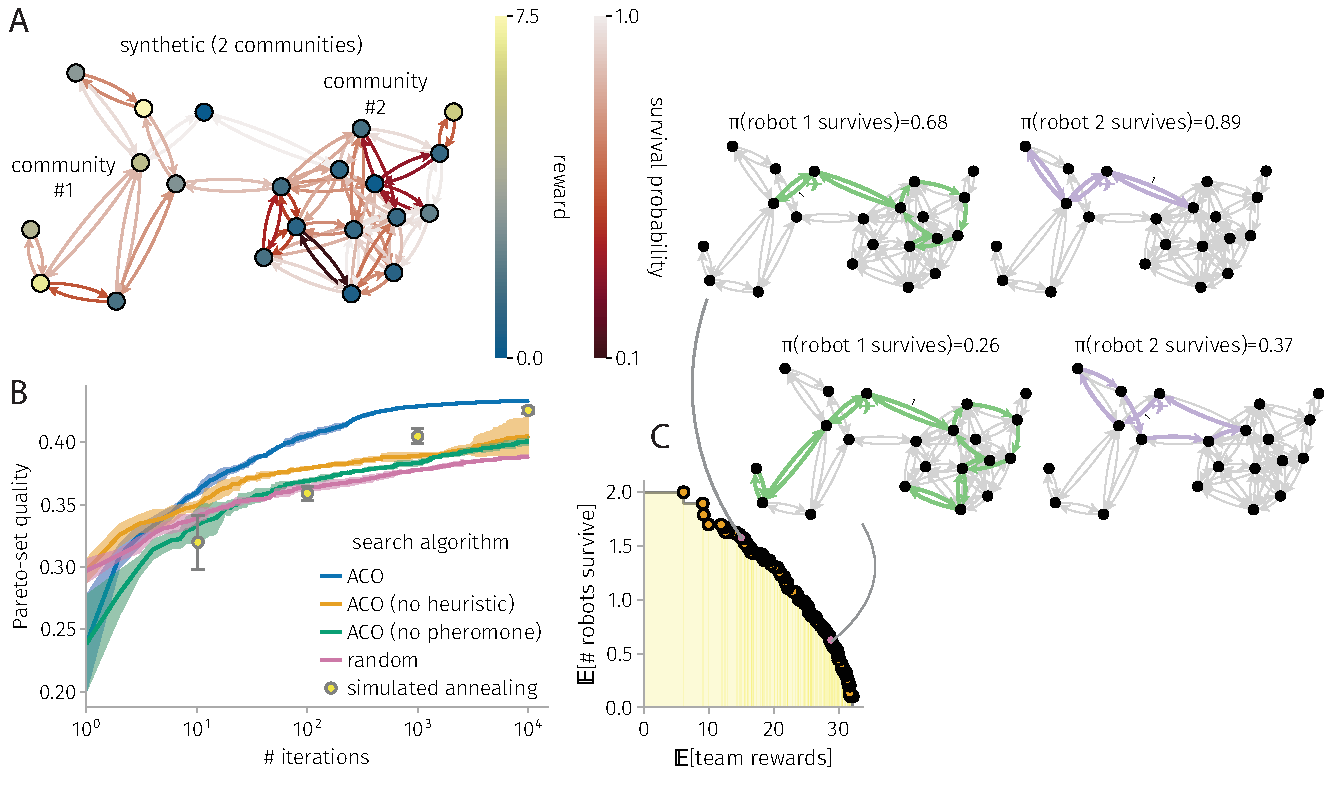
\includegraphics[width=\textwidth]{block_model_results.pdf}
    \caption{
    BOTOHE problem on a random, two-community graph. 
    (A) Problem setup: the graph, node--to--reward map, arc--to--survival-probability map, and robot-team start.
    (B) Search progress of various algorithms (mean, standard deviation over four runs).
    (C) Pareto front of robot-team trail plans at the end of an ACO run and a sample of three plans.
    (D) Pheromone trails at the end of a run of ACO.
    } \label{fig:two_community}
\end{figure}

\paragraph{Setup.}
Fig.~\ref{fig:two_community}A shows the problem setup.
We sampled the two-community graph from a stochastic block model. Community \#1 was assigned 8 nodes; community \#2: 12 nodes.
The probability of joining (both ways) a pair of nodes both in community \#1 and both in community \#2 was 0.3 and 0.4, respectively; and for two nodes in distinct communities, much lower: 0.025.
We assigned a reward to each node by sampling from a distribution based on community membership (both Gaussian and truncated below zero; $\mu_1=5$, $\sigma_1=2$; $\mu_2=1$, $\sigma_2=1/2$).
We sampled arc survival probabilities from a distribution regardless of community membership (Gaussian with $\mu=0.9$, $\sigma=0.3$, truncated below zero and above one). At the base node, $K=2$ robots begin.


\paragraph{Search progress.}
Fig.~\ref{fig:two_community}B shows the search progress of ACO in terms of the normalized area indicator of the Pareto-front of robot-team trail plans over iterations. After 10\,000 iterations, the area indicator for ACO plateaus, suggesting convergence. By comparison, ACO without the heuristics and ACO without pheromone trails perform quite poorly, but better than random search. 
More, ACO outperforms the competitive SA baseline.
Reflecting the competitiveness of SA, at 1\,000 and 10\,000 iterations, SA outperforms ACO without the heuristic and ACO without the pheromone.  
We conclude both the heuristic and pheromone are important in ACO for this problem.

\paragraph{Pareto-front and sample of Pareto-optimal robot-team trail plans.}
Fig.~\ref{fig:two_community}C shows the Pareto-front at the end of an ACO run. The yellow highlighted region represents the [albeit, un-normalized] area indicator that scores the quality of the Pareto-front. 
Three Pareto-optimal robot-team trail plans are highlighted, running down the Pareto front: high expected survival with low expected reward; medium survival and reward; and high reward with low survival. 
    In the high survival, low reward plan, the first robot explores one node of community \#1 then takes a safe closed trail through community \#2, while the other robot visits only three nodes by crossing safe arcs.
   In the medium survival and reward plan, we see more coverage and division of labor among the two robots. The first robot visits five nodes in community \#1 while avoiding the most dangerous arc within it. Meanwhile, the second robot takes a safe closed trail to visit many nodes in community \#2.
   Finally, in the high reward low survival plan, we see even more coverage, some division of labor, and also node-visit redundancy. The first robot visits all nodes in community \#1 while avoiding the most dangerous arc. The second robot visits many nodes in community \#2, then enters community \#1 to reap the rewards therein in the case that the first robot fails. This node-visit redundancy in the team trail plan makes the team reward robust against the failure of one of the robots.

\paragraph{Pheromone trails.}
Finally, Fig.~\ref{fig:two_community}D shows the learned pheromone trails at the end of one of the ACO runs.
First, the distribution of pheromone exhibits a positive skew; most arcs contain only a small amount of pheromone.   
Second, the reward and survival pheromone maps appear similar; the Pearson correlation coefficient between the reward and survival pheromone on an arc is 0.95. 
Third, comparing with the problem setup, the reward pheromone on an arc exhibits a small correlation (coefficient: 0.2) with the reward on its destination node, and the survival pheromone on an arc exhibits a small correlation (coefficient: 0.45) with the survival probability. The lack of a strong correlation further evidences that the pheromone contains information beyond the greedy heuristics that inspect these.
Finally, the asymmetry, where sometimes arc $(v, v^\prime)$ has high pheromone but arc $(v^\prime, v)$ has low pheromone, allows promotion of the robot to take a counter-clockwise closed trail over a clock-wise one.

\paragraph{ACO runtime.} On an Apple M1 iMac, an ACO run on this graph with 21 nodes and 84 arcs consisting of 10\,000 iterations and routing two robots took $\approx$7\,min.



\subsection{Art Museum}
Fig.~\ref{fig:art_museum} shows the results for a BOTOHE problem in the San Diego Art Museum.

\begin{figure}[h!]
    \centering
    	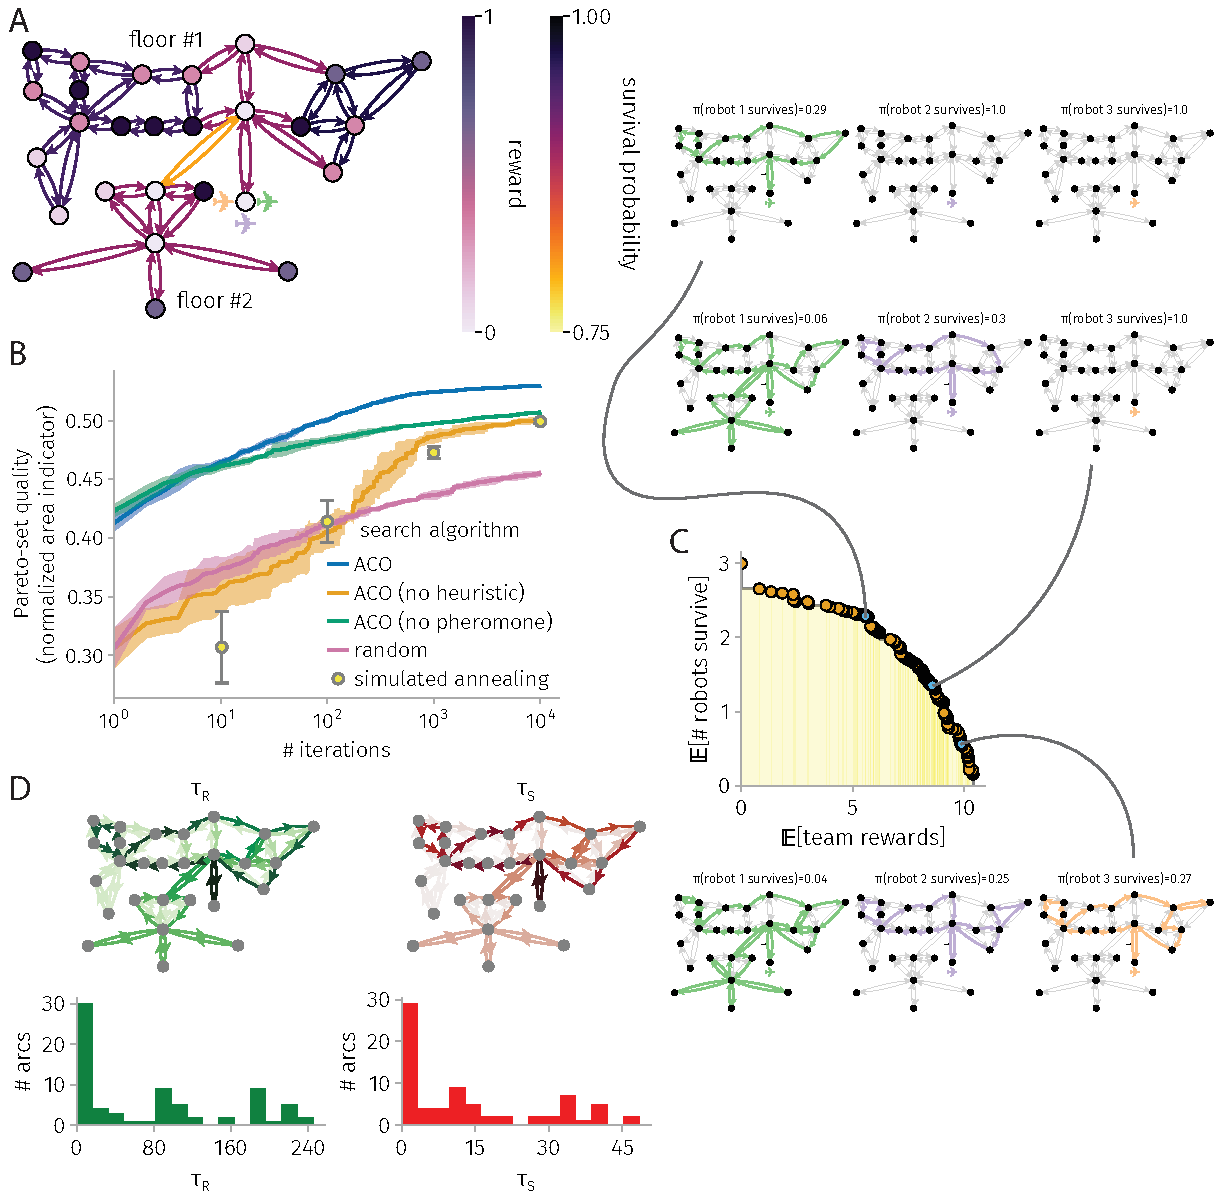
\includegraphics[width=\textwidth]{art_museum_results.pdf}
    \caption{
    BOTOHE problem in the San Diego Art Museum. 
    (A) Problem setup: the graph, node--to--reward map, arc--to--survival-probability map, and robot-team start.
    (B) Search progress of various algorithms. (Mean, standard deviation over four runs.)
    (C) Pareto front of robot-team trail plans at the end of a run of ACO and a sample of three plans.
    (D) Pheromone trails at the end of a run of ACO.
    } \label{fig:art_museum}
\end{figure}

\paragraph{Setup.}
Fig.~\ref{fig:art_museum}A shows the problem setup, where a team of $K=3$ mobile robots are assigned an information-gathering mission in the San Diego Museum of Art. 
% We selected this art museum for (i) its rich connectivity between galleries, giving an interesting example, and (ii) its small size, allowing us to visualize, interpret, and intuit the solution to a BOTOHE problem on it.

We spatially model the art museum as a directed graph $G=(\mathcal{V}, \mathcal{E})$.
The set of 27 nodes $\mathcal{V}$ represents the 23 art galleries/rooms, the outside entrance to the building (base node $v_b$), the main entrance rooms on the first and second floors, and the stairway.
The set of arcs $\mathcal{E}$ represents direct passages/doorways between the rooms or stairs.

Suppose, when a robot visits an art gallery in the museum, it images the art there and transmits this image back to the command center.
The utility of each image to the command center is scored by
the node reward map $r$ assigning rewards of
(i) 2/3 for large galleries,
(ii) 1/3 for medium-sized galleries,
(iii) 1 for small galleries [that, supposedly, contain the most valuable art], and
(iv) 1/10 for the five galleries in corners of the museum or behind the stairway [that, supposedly, contain the least valuable art].

Now, suppose traversing the art museum is hazardous for the robots, owing to
(i) adversarial security guards that (a) seek to prevent the robots from imaging the art and (b) possess the ability attack and/or capture the robots;
(ii) obstacles that the robots could (a) crash into or (b) become entangled in;
(iii) difficult terrain (i.e., the stairs).
To model risks of destruction or capture, we assign survival probabilities $\omega(v,v^\prime)$ for the arc(s)
(i) traversing the staircase of 0.8,
(ii) inside and in/out of the main entrance room of 0.9,
(iii) on the right side of the first floor of 0.97,
(iv) on the left side of the first floor of 0.95,
and
(v) on the second floor of 0.9.
So, the stairway is the most dangerous arc.


The two objectives of the command center are to plan the trails of the robots in the art museum to maximize the (1) expected reward, via robots visiting art galleries, imaging them, then transmitting the images back to the command center, and (2) expected number of robots that return from the mission. 

\paragraph{Search progress.}
Fig.~\ref{fig:art_museum}B shows the search progress of ACO, in terms of the normalized area of the Pareto-front as a function of iterations, in comparison with baselines over 10\,000 iterations. Again, ACO outperforms the competitive SA baseline. Both heuristic and pheromone are important contributors to the ACO search progress, as ablating each diminishes performance significantly. ACO, ACO without heuristics, ACO without pheromone, and SA all perform much better than random search. 

\paragraph{Pareto-front and sample of Pareto-optimal robot-team trail plans.}
Fig.~\ref{fig:art_museum}C shows the Pareto-front at the end of an ACO run along with a sample of three Pareto-optimal robot-team trail plans with different reward-survival tradeoffs. 
In the high-survival, low-reward robot-team trail plan, only a single robot enters the museum to image galleries on the first floor---avoiding the dangerous staircase to the second floor. The other two robots safely stay behind.
In the medium survival and reward plan, the first robot covers much of the first floor and daring traverses the dangerous stairway to visit the second floor to image the galleries there. The second robot covers much of the first floor. The third robot safely stays behind. The redundancy in first-floor coverage by the first two robots makes the team reward robots against the failure of the first (second) robot, as then the second (first) robot could still image most of the galleries on the first floor.
Finally, in the high reward, low survival plan, all three robots enter the museum.
The first robot covers most of the first and, daringly, the second floor. The second and third robots cover most of the first floor. 
 Again, node-visit redundancy, via all three robots covering most of the first floor, makes the team reward robust to the failure of two of the robots on the team.
Note, all three of the robots avoid taking the risk to enter the bottom left corner of the first floor, whose galleries offer only a small reward.

\paragraph{Pheromone trails.}
Fig.~\ref{fig:art_museum}D visualizes the pheromone maps at the end of an ACO run.
Again, the pheromone is very unevenly distributed, with most arcs containing comparably very little pheromone. So, indeed the pheromone expresses a strong preference for which arcs to include in robot trails.
Remarking on pheromone asymmetry, note the clock-wise vs.\ counter-close-wise preferences for some closed trails---to promote pursuit of high-reward nodes earlier in the trails to maximize expected reward.
Interestingly, the reward and survival pheromone on an arc are very strongly correlated (coefficient: 0.99), but they are very weakly correlated with the reward on the destination node and arc survival probability, respectively (coefficients: 0.09 and -0.01). 

\paragraph{ACO runtime.} On an Apple M1 iMac, an ACO run on this graph with 27 nodes and 74 arcs consisting of 10\,000 iterations and routing three robots took $\approx$4\,min.

\subsection{Nuclear Power Plant}
Fig.~\ref{fig:power_plant} shows the results for a BOTOHE problem in the Satsop Nuclear Power Plant.

\begin{figure}[h!]
    \centering
    	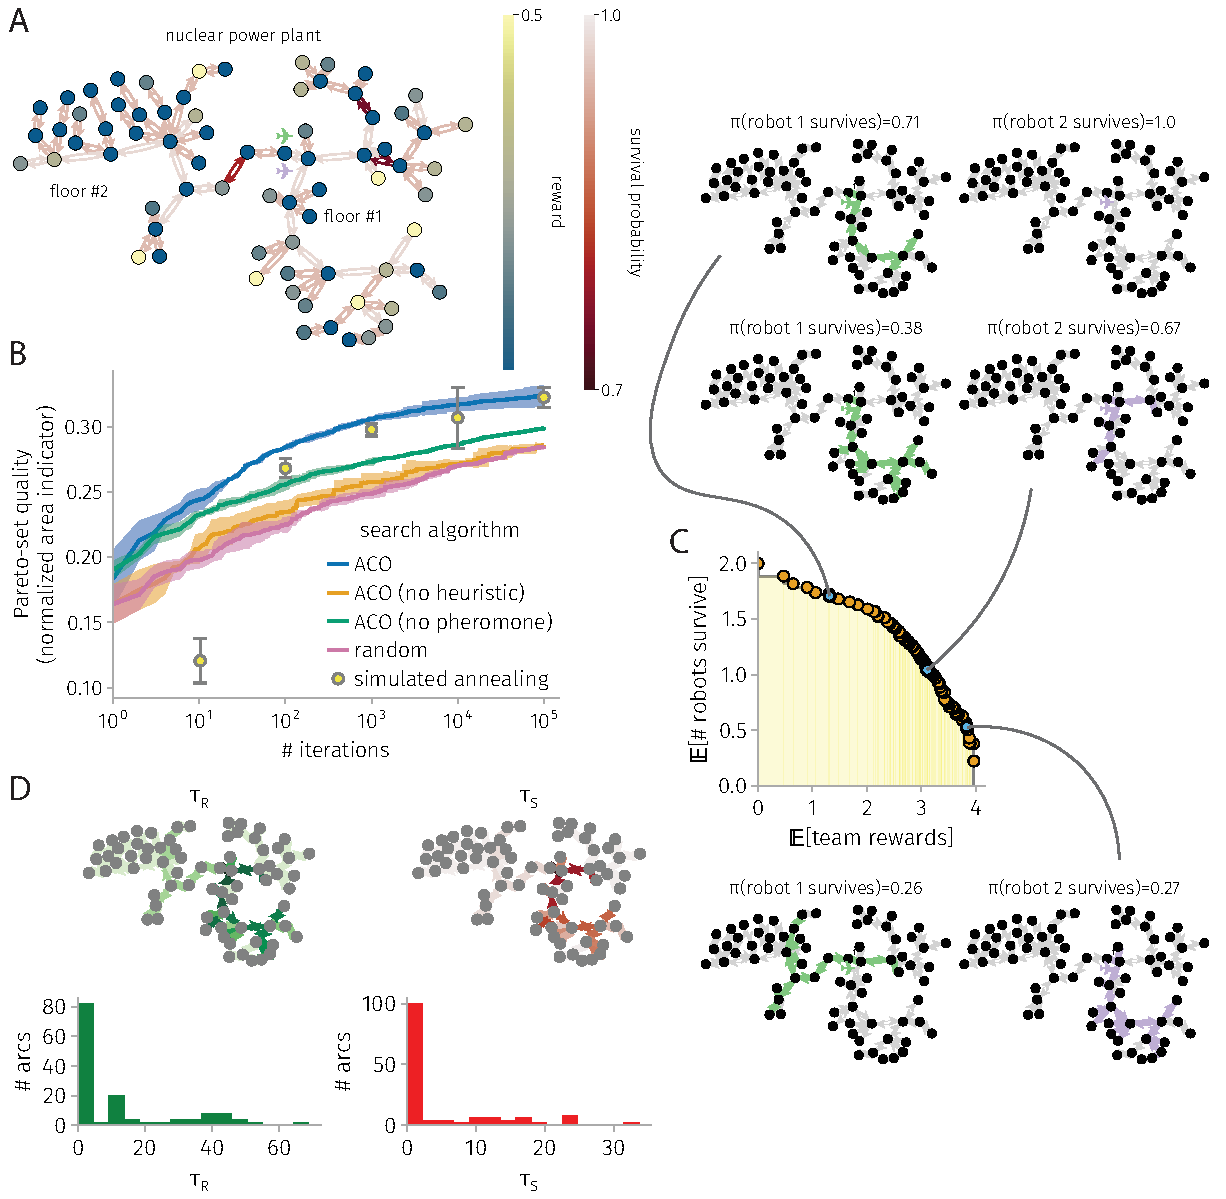
\includegraphics[width=\textwidth]{power_plant_results.pdf}
    \caption{
    BOTOHE problem in the Satsop Nuclear Power Plant. 
    (A) Problem setup: the graph, node--to--reward map, arc--to--survival-probability map, and robot-team start.
    (B) Search progress of various algorithms. (Mean, standard deviation over four runs.)
    (C) Pareto front of robot-team trail plans at the end of a run of ACO and a sample of three plans.
    (D) Pheromone trails at the end of a run of ACO.
    } \label{fig:power_plant}
\end{figure}

\paragraph{Setup.} 
Fig.~\ref{fig:power_plant}A shows the problem setup.
The directed graph represents the unfinished Satsop Nuclear Power Plant in Elma, Washington that was used for the Defense Advanced Research Projects Agency (DARPA) robotics challenge held in 2021 \cite{ackerman2022robots,orekhov2022darpa} (the Subterranean Challenge Urban Circuit \cite{githubdarpasubt}). For the robotics challenge, items were placed at different locations---a [fake] survivor, cell phone, backpack, gas, or vent.
Suppose the mission is for the robots to visit the nodes containing the items to mark, tag, or destroy the artifacts and confirm the presence or status of the survivors, despite the power plant containing obstacles and adversaries patrolling it. 
We assigned 
(1) rewards to each node based on the item present 
(survivor: 0.5; cell phone: 0.3; backpack: 0.2; gas: 0.15; vent: 0.12)
and
(2) arc survival probabilities based on the type of traversal or obstacles present
(open-area traversal: 0.98; doorway traversal: 0.95; stairway traversal: 0.8; obstacle: 0.75). A team of $K=2$ robots begin at the entrance to the power plant on the first floor.

\paragraph{Search progress.}
Fig.~\ref{fig:power_plant}B shows the search progress of ACO---the normalized area under the Pareto-front of robot-team trail plans as a function of iterations---in comparison with baselines, over 100\,000 iterations. 
ACO is the best-performing search algorithm over 10, 100, 1\,000, and 10\,000 iterations; but, at 100\,000 iterations, the performance of SA and ACO are indistinguishable. 
Again, ablating the pheromone or the heuristic in ACO leads to significantly poorer performance; both the pheromone and heuristic are important for guiding ACO's search. Interestingly, ACO without the heuristic is not much better than random search, suggesting synergy between the pheromone and heuristic. 

\paragraph{Pareto-front and sample of Pareto-optimal robot-team trail plans.}
Fig.~\ref{fig:power_plant}C shows the Pareto-front and a sample of three Pareto-optimal robot-team trail plans at the end of an ACO run.
In the low-reward, high-survival plan, the first robots visits the bottom portion of the first floor of the power plant containing the highest rewards while the second robot stays behind for safety.
In the medium-reward and -survival plan, the two robots visit highly-overlapping portions of the first floor.
In the high-reward and low-survival plan, the first robots daringly visits the second floor, taking the dangerous staircase, then also visits three nodes on the first floor before returning. The second robot visits most of the bottom portion of the first floor containing the highest rewards.
Interestingly, the trail plans of the two robots contain little redundancy. And, none of the plans send the robots to the upper portion of the first floor where many nodes offer no rewards yet there are two very dangerous arcs.

\paragraph{Pheromone trails.}
Fig.~\ref{fig:power_plant}D shows the reward and survival pheromone trails at the end of an ACO run.
The pheromone expresses strong preferences for the robot trails to be constructed with certain arcs, indicated by the highly skewed-right distributions.
The reward and survival pheromone on an arc are quite correlated (coefficient: 0.97), with a good degree of correlation with the reward on the destination node and arc survival probability, respectively (coefficients: 0.3, 0.25).

\paragraph{ACO runtime.} On an Apple M1 iMac, an ACO run on this graph with 73 nodes and 144 arcs consisting of 100\,000 iterations and routing two robots took $\approx$30\,min.




\section{Conclusions and Discussion}
Teams of mobile robots---ground (wheeled \cite{chung2016wheeled}, legged \cite{wieber2016modeling}, or snake-like \cite{walker2016snake}), underwater \cite{choi2016underwater}, or flying \cite{leutenegger2016flying} robots---have many applications: gathering information, delivering resources, locating and mapping CBRN hazards, fighting forest fires, tracking targets, patrolling for wildlife poachers, inspecting infrastructure, etc.
In these applications, the environment may contain hazards or adversaries that can destroy, immobilize, or capture a robot or damage a robot's sensors or actuators, compromising its functionality for the mission \cite{trevelyan2016robotics}.
Hazards could emanate from the presence of radiation or corrosive chemicals, extreme temperatures, smoke that obscures obstacles, rough terrain or seas, high winds, dust and debris, etc.
For a robot team to perform well on a shared, high-level objective in a hazardous environment, the robots must coordinate their trails while considering the risks of failure, balancing the rewards from visiting locations against the risks to reach them, and including redundancy to make achievement of the objective robust to robot failures. 

Heavily inspired by the Team Surviving Orienteers Problem \cite{jorgensen2018team,jorgensen2017matroid,jorgensen2024matroid}, we framed the bi-objective team orienteering in a hazardous environment (BOTOHE) problem.
A team of robots are mobile on a directed graph whose nodes offer rewards when visited by a robot and arcs are dangerous to traverse.
We sought the Pareto-optimal set of robot-team trail plans that trade maximizing the expected team reward with maximizing the expected number of robots that survive. 
With this approach, a human decision-maker can inspect the Pareto-front to see reasonable choices of reward-survival tradeoffs. Then, this decision-maker can make an informed selection of a Pareto-optimal robot-team trail plan for the mission, invoking their values placed on reward vs. robot-survival.

We employed bi-objective ant colony optimization to search for the Pareto-optimal team trail plans, guided by both (i) pheromone trails serving as a collective memory about which arcs led to Pareto-optimal robot team trail plans and (ii) TOHE problem-specific heuristics. We deployed ACO on three BOTOHE problem instances: (1) a synthetic mission on a random two-community graph; (2) an information-gathering mission in an art museum; and (3) an artifact-marking and status-checking mission in a nuclear power plant involved in a DARPA robotics challenge.
Despite lacking theoretical guarantees to find the Pareto-optimal set, ACO was effective, easy to implement, and can be readily adapted to handle extensions to the TOHE problem. 
We found ACO to consistently outperform or, at worst, perform indistinguishably from, bi-objective simulated annealing.
Ablating the heuristics or pheromone in ACO both significantly degraded the quality of the Pareto-set of robot-team trail plans. 
This underscores the importance of pheromone and the heuristics for guiding the simulated ants in ACO to search for Pareto-optimal robot-team trail plans. 
Finally, inspecting high-survival \& low-reward, medium reward \& survival, and high-reward \& low-survival Pareto-optimal robot-team trail plans for each case study provided intuition about the BOTOHE problem specification and demonstrated the practical utility of our work for planning the trails of a team of robots mobile in a hazardous environment.

\paragraph{Future work.}
%Much future work remains for path-planning of robots in adversarial/hazardous environments.
% harvesting the reward is dangerous. not visiting. 
For the BOTOHE, we wish to devise and benchmark ACO variants that:
(i) handle the online setting, where the robots adapt their planned trails during the mission, in response to observed failures of robots; 
(ii) handle the dynamic setting, where, over time, arcs may become more or less dangerous to traverse and nodes may increase or decrease the reward they offer;
%  while the robots are following their planned trails, calling for on-the-fly modification of the remains of the planned trails in response to the new objective function; 
(iii) run a local search algorithm to improve the robot trails the ants found after each iteration and thereby accelerate convergence \cite{dorigo2006ant}, 
(iv) concurrently extend the planned trails of the robots instead of sequentially allocating their planned trails robot-by-robot \cite{ke2008ants}, and 
(v) employ multiple ant colonies \cite{iredi2001bi}.

Interesting and practical extensions of robot-team orienteering in adversarial/hazardous environments abstracted a graphs include treating (some of these ideas from Ref.~\cite{jorgensen2018team}): 
(i) a heterogenous team of robots with different (a) capabilities to harvest rewards from nodes and (b) survival probabilities for each arc traversal owing to e.g.\ stealth;
(ii) more complicated reward structures, e.g., time-dependent, stochastic, non-additive (correlated \cite{yu2014correlated}), multi-category, or multi-visit rewards;
(iii) fuel/battery constraints of the robots via nodes representing refueling, recharging, or battery-switching stations \cite{asghar2023risk,khuller2011fill,liao2016electric,yu2019coverage}; 
(iv) constraints on the rewards a robot can harvest e.g.\ for resource delivery applications where each robot holds limited cargo capacity \cite{coelho2014thirty};
(v) non-binary surviving states of the robots due to various levels of damage;
(vi) non-independent events of robots surviving arc-traversals;
(vii) risk metrics different from the expected value \cite{majumdar2020should}.
% TODO: cite green vehicle routing

Another interesting direction is to update uncertain survival probabilities associated with the edges of the graph from data over repeated missions (an inverse problem \cite{burton1992instance}) under a Bayesian framework. 
Specifically, suppose we are uncertain about the survival probability $\omega(u, v)$ of each arc $(u,v)$. We have a prior distribution on each $\omega(u,v)$. Then, when a robot survives or gets destroyed while following a planned trail during a mission, we update this prior distribution with this data. 
The trail-planning of the robots over sequential missions may then balance (a) exploitation to harvest the most reward and take what appear to be, under uncertainty, the safest trails and (b) exploration to find even safer trails.

\section*{Acknowledgements} CMS acknowledges the Office of Naval Research Summer Faculty Research Program.

\bibliographystyle{unsrt}
\bibliography{refs}


\end{document}  
